
\documentclass[refcompress,eversion,noinfo]{ICTthesis}

%\usepackage{amssymb}
%\usepackage[thmmarks]{ntheorem}
\usepackage{amsmath}
\usepackage{amsthm}
\usepackage{tabularx}
\usepackage{longtable}
\usepackage{color}
\usepackage{colortbl}
\usepackage{graphicx}
\usepackage{subfigure}
\usepackage{epsfig}
\usepackage{enumerate}
\usepackage{multirow}
\usepackage{amsfonts}
\usepackage{algorithm}
\usepackage{algorithmicx}
\usepackage{algpseudocode}
\usepackage{tikz}
\usetikzlibrary{decorations.pathreplacing}
%\usepackage[margin=1.1in]{geometry}

\graphicspath{{figures/}}
%\linespread{1.3}

\definecolor{bkcolor1}{gray}{0.95}
\definecolor{bkcolor2}{gray}{0.85}
\newcommand{\bkcommand}[1]{\colorbox{bkcolor1}{$\mathtt{\backslash}$\texttt{#1}}}
\newcommand{\textgraph}[1]{\raisebox{-1ex}{\includegraphics[width=1.5em]{#1}}}

%\floatname{algorithm}{算法}
\renewcommand{\algorithmicrequire}{\textbf{Input:}} 
\renewcommand{\algorithmicensure}{\textbf{Output:}}

%\theoremsymbol{$\square$}
%\newtheorem*{proof}{证明}
\theoremstyle{plain}
%\theoremsymbol{}
%\theoremseparator{:}

\newtheorem{theorem}{定理}
\newtheorem{lemma}{引理}
\newtheorem{proposition}{命题}
\newtheorem{corollary}{推论}
\newtheorem{definition}{定义}

\newcommand{\upcite}[1]{\textsuperscript{\cite{#1}}}

\begin{document}
\ICTfrontmatter

\begin{abstract}

随着互联网的普及,越来越多的人加入社交网络展示自己的生活。
社交网络的即时性使得信息和谣言可以在网络上很快传播,在线社交网络的病毒式营销成为广告的新趋势。
由此启发,许多工作研究了怎样最大化信息的传播,也就是所谓的{\it 影响力最大化}问题。
深入理解信息在社交网络中的传播机制,以及如何控制疾病的传播、舆论的导向和营销策略的选择
已经成为研究热点,影响力最大化问题和传播模型已成为许多领域涉及的重要内容。


影响力最大化旨在从网络中选择$k$个种子节点,使得这$k$个种子节点通过传播模型产生的影响传播范围最大。
这个问题已经被广泛研究,但是大多的工作专注于次模的影响力传播模型。
受现实的传播现象启发,本论文探讨了非次模设定下的影响力最大化问题。
在通用阈值模型框架下,本论文定义了一类被次模上下界紧紧夹住的非次模阈值函数({\it $\varepsilon$-次模逼近函数}),
讨论图中有部分节点是$\varepsilon$-次模逼近阈值函数的情况。
我们首先通过NP完全归约证明了不可近似性结论:
即使$n$个节点的图中只有$n^{\gamma}$个$\varepsilon$-次模逼近节点,
也不存在近似比为$1/n^{\frac{\gamma}{c}}$的算法,除非P = NP,其中$\gamma \in (0,1)$且$c$是依赖于$\varepsilon$的常数。
然后我们针对有$\ell$个$\varepsilon$-次模逼近节点的图设计了近似比为$(1-\varepsilon)^{\ell}(1-\frac{1}{e})$的算法。
最后我们在一系列真实的社交网络数据上做了对比试验,实验结果表明我们提出的近似算法要比其他基准算法效果更好。

此外本论文研究了另一种阈值函数——$k$-激活函数,
这种阈值函数对应着一个节点只有在其$k \geq 2$ 个邻居都被激活后自己才会被激活的传播模型。
在Kleinberg的小世界网络模型中,强连接被认为是底层网格上确定的边,而弱连接指连接相距较远的节点之间的随机边。
节点$u$和节点$v$通过一条弱连接相连的概率正比于$1/|uv|^\alpha$,
此处$|uv|$是节点$u$和$v$之间的网格距离,而$\alpha\ge 0$是小世界网络模型的参数。
本论文类比Kleinberg的分散式路由,提出了基于$k$-激活阈值函数的路由(简称{\it $k$-激活路由}),
同时对Kleinberg小世界网络上$k$-激活路由时间进行了理论分析,
求得$k$-激活路由的路由时间在所有$\alpha$范围内的$n$的多项式的下界($n$是网络中节点的个数)。



\keywords{社交网络, 社会影响力, 小世界网络, 影响力最大化, 路由}

\end{abstract}

\begin{englishabstract}

With the prevalence of Internet, more and more people join social network to show their daily life.
Information and rumors could spread fast in social networks because of its instantaneity, and viral marketing on online social network becomes a new trend of advertising. 
Motivated by this, plenty of research focuses on how to maximize the information propagation, which is called the {\it influence maximization} problem.
Deeply understanding the propagation mechanisms of social networks as well as controlling disease spread,
guiding public opinion and marketing strategy have become heated research topics.
Many recent works that involve various fields focused on the influence maximization in social networks and information propagation model.

Influence maximization is the problem of selecting $k$ nodes in a social network to maximize their influence spread.
The problem has been extensively studied but most works focus on the submodular influence diffusion models.
In this thesis, motivated by empirical evidences, we explore influence maximization in the non-submodular regime.
In particular, we study the general threshold model in which a fraction of nodes have non-submodular threshold
	functions, but their threshold functions are closely upper- and lower-bounded by some submodular
	functions (we call them $\varepsilon$-almost submodular).
We first prove a strong hardness result with NP-complete reduction: there is no $1/n^{\frac{\gamma}{c}}$ approximation for influence maximization (unless P = NP)
	for all networks with up to $n^{\gamma}$ $\varepsilon$-almost submodular nodes, where $\gamma$ in $(0,1)$ 
	and $c$ is parameter depending on $\varepsilon$.
We then provide $(1-\varepsilon)^{\ell}(1-\frac{1}{e})$ approximation algorithms when the number of $\varepsilon$-almost submodular nodes is $\ell$.
Finally, we conduct experiments on a number of real-world datasets, and the results demonstrate that our approximation algorithms
	outperform other benchmark algorithms.

Besides we study the threshold function ---- $k$-activation function, 
which corresponds to a propagation model where each node is activated only
after $k \ge 2$ neighbors of the node are activated.
In Kleinberg's small-world network model, strong ties are modeled as deterministic edges in the
underlying base grid and weak ties are modeled as random edges connecting remote nodes.
The probability of connecting a node $u$ with node $v$ through a weak tie is proportional to
$1/|uv|^\alpha$, where $|uv|$ is the grid distance between $u$ and $v$ and $\alpha\ge 0$ is the
parameter of the model.
We investigate a new propagation phenomenon closer to decentralized routing proposed by Kleinberg,
which is called the routing under $k$-activation threshold function (or {\it $k$-activation routing}).
Meanwhile the thesis studies complex routing in Kleinberg's small-world networks and proves that
routing time is lower bound by a polynomial in $n$ (the number of nodes in the network) for all range of $\alpha$.

\englishkeywords{Social Network, Social Influence, Small World Network, Influence Maximization, Routing}

\end{englishabstract}

\ICTmainmatter

\chapter{绪论}
二十一世纪互联网发展迅猛,人与人之间不再仅仅只能当面交流,电子邮件、电话和即时通讯软件让人们之间的沟通更迅捷。与此同时,社交网站也在兴起,积累了越来越多的用户。在社交网络中,信息传播得更快,在社交网络中的营销手段会比传统营销获得更大的收益,有一些相关学者开始关注社交网络中的信息传播现象。


\section{课题研究的背景与意义}
社交网络(Social network)是由许多节点构成的一种社会结构。节点通常是组织和个人,节点之间的连接代表社会个体之间的关系,经由这些社会关系,把从偶然相识的泛泛之交到紧密结合的家庭关系的各种人们或组织串连起来。“社交网络”的概念从心理学、社会学、人类学、数学、统计学、计算机科学等不同领域不断深化,形成了一套系统的理论、方法和技术。在21世纪,人们获取信息的途径不再局限于报纸、广播、电视和当面交谈,随着Facebook,Twitter和Weibo等社交工具的广泛应用,社交网络已经成为重要的信息传播工具。在社交网络上,人们通过添加好友和关注建立人与人之间的连接,通过发消息、短文章、分享连接进行交流。信息在社交网络上可以沿着人与人之间的连接很快传播,很多新闻、广告在社交网络上可以很快的覆盖到绝大多数用户,这相对于传统的媒体介质有很大的优势。在互联网时代,社交网络成为了重要的信息传播工具,利用社交网络进行产品或信息的推广是很有力的手段。在实际应用场景中,会有这样的案例,某公司准备发售一款新产品,想要在社交网络上做一些免费体验活动,希望免费体验的人可以把产品较好的口碑在朋友间扩散出去,最后达到产品推广的目的。随之产生了这样一个优化问题,给定了网络结构和信息传播的模型之后,如何选定k个人作为种子,使得这$k$个人最后影响的范围最大,这就是社会网络影响力最大化\cite{Kempe2003maximizing}。这个问题被证明是NP难的,而且因为社交网络的规模很大,暴力的枚举所有种子集合很不现实,设计高效的有近似比保证的算法是很有需求的。

社会网络影响力最大化在被Kempe, Kleinberg和Tardos\cite{Kempe2003maximizing}提出并公式化之后,已经在学术界引起了广泛的关注,近年来很多学者都在做相关研究,涉及到病毒营销、媒体广告和谣言传播等方向。很多学者提出了比较有效的算法\cite{Kempe2003maximizing,Leskovec2007celf,Chen2009efficient,chen2010sharpphard,tang2014newrrset},这些算法大部分是采用了独立级联(Independent Cascade)或者线性阈值(Linear Threshold)[1]的信息传播模型。在这两种传播模型下,影响力函数是次模(Submodular)的,这时候可以使用贪心策略得到1-1/e近似的算法。此外,在一个更一般的通用阈值(General Threshold)\cite{Kempe2003maximizing}传播模型下,每个用户的阈值函数(Threshold Function)不再是简单的把边的权值相加,而是一个集合函数。伯克利的学者Elchanan和Sebastien\cite{Mossel2007sub}证明了阈值函数是次模的时候整体的影响力函数也是次模的,也就意味着局部的次模性质会导致全局的影响力函数的次模性。

然而,在真实的社交网络中,非次模的影响力传播现象经常出现。Backstrom\cite{backstrom2006group}研究了LiveJounral和DBLP两个大型的社交网络数据,他绘制了个体加入某个社区的意愿与她的已经加入该社区好友数量的关系图。论文的图中可以看到意愿曲线整体上是上凸的,但是在最开始几个点有明显的下移。杨洋\cite{yang2016role}等人观测了另一个社交网络Flickr,他们主要观察人的情绪变化被他带有情绪的朋友的影响。他们指出人变快乐的可能性和已经快乐的好友数量是一个超线性关系,尤其是那些影响力比较大的朋友。这些结果都指出现有的基于独立级联或者线性阈值模型的算法在真实的社会网络种可能并不能使用。很多非次模的传播模型已经被证明很难近似,像谣言和疾病的传播,需要社交网络中的个体在被影响邻居的数量超过某个阈值的时候才会被影响,这种模型也是通用阈值模型的变种,被称作固定阈值模型(Fixed Threshold Model)。在固定阈值模型下,社交网络影响力最大化问题是NP-hard的,而且有很强的不可近似性\cite{Kempe2003maximizing}。与此同时,如果考虑寻找能达到给定影响力目标的最小种子集合问题,也就是社会影响力最小化种子集合问题,陈宁也证明了这个问题也很难被近似\cite{Chen2008approximability}。学者们倾向于相信是次模性质帮助我们在社会影响力最大化问题中找到了比较好的近似算法。但是我们可以使用次模性质到什么程度呢?如果影响力传播过程仅仅是稍微偏离了次模性质,那么是否还有可能仍然设计一个近似比足够好的算法呢?这些问题现在仍然是需要解决的。

与此同时,固定阈值模型下的问题还有一些仍未被探索,前面说到的影响力传播,实际上只关心最后影响的人的数量,而不关心传播的时间和步数。考虑给定种子和目标节点的情况下,在不知道整体网络结构时,如何才能通过影响最少的人而影响目标?其实可以规定一个时间片只能影响一个人,问题就变成了社会网络里面,在固定阈值模型下,从给定的种子到目标点需要经过多少步跳转或者多少个时间片。这就是从另一个角度来研究社会影响力,从影响力传播的时间而不是影响的范围。此外,这里研究的是路由现象,就像IP包在路由网络里转发一样,IP包只知道最后的目的地,并不知道每一步应该具体怎么转发,也不能在每一个路由器群发,只能一步一步的跳转。我们研究的就是在社交网络里面的路由现象,跟传统路由的区别有两个,一个是社交网络的结构,没有路由表;另一个是每个节点被影响的邻居超过一定阈值时才能被影响到。在文章里,称类似IP包跳转的现象为简单路由,把影响需要阈值的路由为复杂路由。

社交网络是一个小世界网络,人与人之间的最短路很短。二十世纪60年代,美国哈佛大学社会心理学家斯坦利·米尔格伦(Stanley Milgram)做了一个连锁信实验\cite{Milgram1967small}。他将一些信件交给自愿的参加者,要求他们通过自己的熟人将信传到信封上指明的收信人手里,他发现,294封信件中有64封最终送到了目标人物手中。而在成功传递的信件中,平均只需要5次转发,就能够到达目标。也就是说,在社会网络中,任意两个人之间的“距离”是6。这就是所谓的“六度分隔”理论(Six Degrees of Separation)。尽管他的实验有不少缺陷,但这个现象引起了学界的注意。小世界网络就是对这种现象(也称为小世界现象)的数学描述。用数学中图论的语言来说,小世界网络就是一个由大量节点构成的图,其中任意两点之间的平均路径长度比节点数量小得多。除了社会网络以外,小世界网络的例子在生物学、物理学、计算机科学等领域也有出现。许多现实中的图可以由小世界网络作为模型。万维网、公路交通网、脑神经网络和基因网络都呈现小世界网络的特征。本文采用经典的Kleinberg网络\cite{Kleinberg2000small},这是一个基于二维网格的小世界网络,网格的边被称为人与人之间的强链接,而同时每个节点会发出若干条随机的弱连接。Kleinberg指出当模型的参数$\alpha$等于网格的维度时,贪心路由算法有很高的效率。这里的贪心路由算法是指在每一步,当前节点把消息传递给他的邻居里面距离目标节点曼哈顿距离最小的节点。这个路由算法的需要的跳转数也符合之前Milgram的实验结果,从理论上支持了小世界现象。Kleinberg进一步指出当模型的参数$\alpha$不等于网格的维度时,所有的路由算法都不能很快地把信件送达到目标手中。本文关注的是小世界网络中复杂路由的速度,复杂路由每一步激活的过程就是固定阈值模型,也是通用阈值模型范畴下的子问题。


\section{国内外研究现状}
在Kempe, Kleinberg和Tardos\cite{Kempe2003maximizing}提出影响力最大化的问题之后,近些年来很多工作陆续研究了这一问题\cite{bharathi2007competitive,Leskovec2007celf,Chen2009efficient,chen2010sharpphard,Goyal2011simpath}。其中值得注意的是Leskovec\cite{Leskovec2007celf}在07年提出了一种lazy-forward的优化方法,利用了影响力函数$\sigma(\cdot)$的次模性质,本轮计算的$\Delta_x\sigma(\cdot)$随着轮次增加只会递减而无需再次计算,避免了对种子集合影响力的重复计算,极大地提升了贪心算法的速度。陈卫在09年\cite{Chen2009efficient}和10年\cite{chen2010sharpphard}连续提出了高性能的启发式算法,可以在DBLP等有六十万节点百万条边的大型网络上运行,而且算法效果几乎和贪心算法持平。算法的主要思想是把影响传播过程近似分解为影响力路径,计算每条影响力路径的概率,最后近似得到影响力大小。在14年,Borgs等人\cite{borgs2014rrset}提出了逆向可达集合(Reverse Reachable Set)的技术来加速计算一个集合影响某个节点的概率,然后把问题转化为最大集合覆盖问题,并且依靠这个技术首次把影响力最大化算法的复杂度降到近线性。Tang等人\cite{tang2014newrrset}工程化的实现了Borgs提出的近线性算法并且在具有十亿条边的Twitter网络上测试了算法的性能和效率。紧接着,Tang\cite{tang2015influence}和Nguyen\cite{mtai2016sigmod}进一步提升了基于逆向可达集合的贪心算法的效果,主要是改进了分析的办法,利用更少的逆向可达集合来保证算法的运行。这一系列的影响力最大化相关工作大部分都是利用了次模性质来加速了近似算法,得到$1-1/e$的近似比。

种子集合最小化是和影响力最大化对立的问题,是找到一个影响力超过给定阈值的最小种子集合的问题。陈宁在08年\cite{Chen2008approximability}给出了固定阈值模型下很强的不可近似结果。固定阈值模型也是通用阈值模型的特例,固定阈值模型的阈值函数是在阈值处有一个从0到1的突变。Goyal在12年\cite{goyal2012minimizing}提出了一个双向近似的种子集合最小化的贪心算法。最近,张鹏\cite{zhang2014prob}在KDD14上第一次提出了种子集合最小化的一个概率变种模型,主要是关注给定的种子集合的影响力能否以一定的概率保证达到给定阈值,而之前的工作大部分只关心最终影响力的期望的大小。


非次模问题的最优化是近些年研究的另一个关注点,次模问题的最优化已经有比较成熟的结果,非次模问题还有很多需要探索。堵丁柱\cite{du2008analysis}在08年提出了约束次模和偏移次模两个技术用来研究非次模优化的贪心算法近似比,并且在Steiner Tree问题上给了细致的分析。Horel等人\cite{Horel2016sub}刚刚在NIPS16上研究了一类非次模但是和次模函数很接近的函数优化问题,他们假设函数值可以从一个数据库里面不断获取,关注的是找到函数h最大值点的同时需要从数据库询问的次数。

对于Kleinberg小世界网络[10],Nguyen和Martel在2004年\cite{Martel2004analyzing}和2005年\cite{Nguyen2005analyzing}分析了小世界网络中简单传播时间的上下界,也就是小世界网络的半径。他们指出对于二维网格在$\alpha<4$时,Kleinberg’s model都是一个小世界网络,网络中的任意两个节点之间的最短路径是网络中节点个数的对数级。Ghasemiesfeh等人\cite{Ghasemiesfeh2013complex}在2013年首次给出了复杂传播的理论分析,他们研究了一个节点只有在至少$k$个邻居被激活时才能激活的$k$-复杂传播。他们的理论分析支持了弱连接在复杂传播过程中作用较小的观点,同时指出复杂传播的速度很大程度上取决于弱连接的分布,在15年\cite{ebrahimi2015complex}他们进一步探索了复杂传播和聚集系数$\alpha$的关系。Gao等人在16年\cite{gao2016gt}进一步研究了阈值模型下每个节点的阈值服从一个分布时$k$-复杂传播的一些问题。




\section{本文所做的工作}
社交网络影响力传播的非次模现象很普遍,本文研究非次模问题里一个比较特殊的例子并且深入下去,从通用阈值模型入手。
本文首先提出了$\varepsilon$-次模逼近和$k$-激活这两个非次模阈值函数,然后分别证明了$\varepsilon$-次模逼近模型下影响力最大化难以近似和$k$-激活模型下复杂路由速度很慢,最后研究了$\varepsilon$-次模逼近节点较少时的影响力最大化近似算法,并且设计了模拟实验。主要工作成果如下:


\begin{enumerate}
\item  提出$\varepsilon$-次模逼近函数和$k$-激活阈值函数。
\item  通过构建机关和级联机关,证明了$n$个节点的图中图中有$n^{\gamma}$个$\varepsilon$-次模逼近节点时,影响力最大化很难被近似。通用阈值模型在每个节点的阈值函数都是次模的时候,影响力函数也是次模的\cite{Mossel2007sub}。$\varepsilon$-次模逼近函数不是次模,但又和次模函数相距很近,但是本文证明了$n^{\gamma}$个$\varepsilon$-次模逼近节点足以让整体影响力函数偏移次模很远,阈值函数一点很小的偏移会导致整体影响力函数不可近似。
\item  通过对Kleinberg小世界网络中弱连接分布的深入研究,证明了$n$个节点小世界网络中,对于任意范围内的聚集系数$\alpha$,$k$-激活路由时间是$n$的多项式的(polynomial)。对比简单传播、简单路由和复杂传播较快的速度($n$的对数多项式级),我们的结果显示复杂路由更加困难。
\item  对于$\varepsilon$-次模逼近节点较少的图,设计了近似算法,分析了算法的性能并给出近似比保证。对于只有$n$的对数级$\varepsilon$-次模逼近节点的图中,算法的近似比比较好。然后借助蒙特卡罗模拟,设计实验模拟影响力传播过程。实现了本文提出的算法和几种常见算法,发现本文提出的算法速度快而且性能和其他算法相比有较大的提升。
\end{enumerate}

\section{论文组织结构}
论文组织结构如下:

第一章 绪论

介绍课题的研究背景,阐述了影响力最大化和小世界现象的研究背景以及国内外研究现状,提出本文的研究目标和主要工作内容。

第二章 相关技术综述

介绍本文工作涉及到的主要相关理论及模型,重点分析了Kleinberg小世界网络以及复杂传染病的相关知识,
然后介绍了蒙特卡洛模拟的相关技术。

第三章 蒙特卡洛模拟及实验结果分析

首先给出了基于Kleinberg小世界网络的蒙特卡洛模拟实验的设计,然后介绍实验目的和步骤,
最后给出实验结果和分析过程。

第四章 复杂传播的研究

首先给出复杂路由的主要结论,然后给出证明的框架和基于框架给出完整的证明。
最后把结论扩展到$k$-复杂传播并与简单传播进行比较。


第五章 复杂路由的研究

给出复杂路由的结论及完整的证明过程,然后探讨一步允许感染$m$个节点的复杂路由,建立起复杂传播和复杂路由的关系。

第六章 总结与展望

在最后的总结与展望中,首先整体给出了文章的结论,然后对比本文结果和已有结果,深入讨论了复杂传播和简单传播的内在差别。
然后指出已有工作的不足,并对下一步的工作进行展望。

\chapter{小世界网络及影响力传播基础}
在本章中,首先介绍Kleinberg小世界网络模型和影响力传播模型,然后基于影响力传播模型介绍影响力最大化算法的相关工作。最后介绍如何用蒙特卡罗模拟估算影响力大小。

\section{Kleinberg小世界模型}
Kleinberg的小世界模型是一个由$n$个节点的集合$V$生成的随机图。
$n$个节点分布在一个$\sqrt{n} \times \sqrt{n}$的二维网格上\upcite{Kleinberg2000small},为了方便,
我们把网格的上边界和下边界连接起来,同时也把网格的左边界和右边界连接起来。
这样二维网格就变成了“环面”,网格中每个节点的位置都是对称的。
网格上两个节点$u$和$v$之间的曼哈顿距离(Manhattan distance)$|uv|$是
在网格上$u$到$v$的最短路径的长度。

这个随机图上有两种类型的边:{\it 强连接}和{\it 弱连接}。
强连接是任意两个曼哈顿距离不超过$p$的节点之间生成的无向边,这里$p \geq 1$是一个模型的常数。
弱连接指连接节点$u$和网格上可能相距较远的节点$v$之间的随机边。
每个节点$u$会有$q$条互相独立的弱连接边,$u$的第$i$条弱连接边以$v$为终点的概率
正比于$1/{|uv|}^\alpha$,$\alpha\geq 0$是小世界模型的参数。
我们用$1/{|uv|}^\alpha$乘以归一化因子$\mathcal{Z} = 1/\sum_{v\in V}|uv|^{-\alpha}$(在环形网格上,这个值对于任意的节点 $u\in V$都相等),这样就得到了弱连接的概率分布函数。
最初Kleinberg描述的网络模型\cite{Kleinberg2000small}中,$u$到$v$之间的弱连接被认为是有向边,这样的网络被称为{\it 有向Kleinberg小世界网络模型}。
而有些研究工作\cite{Ghasemiesfeh2013complex}中弱连接被认为是无向的,这样的网络被称为{\it 无向Kleinberg小世界网络模型}。
两个模型在本文中都被讨论了,在分析复杂传染病的传播时,我们为了和以前的工作保持一致,
采用无向Kleinberg小世界网络模型。
分析复杂传染病的路由时,我们使用有向Kleinberg小世界网络模型。

\section{影响力传播模型}
社交网络被定义为一个有向图$G=(V,E)$,其中$V$是所有节点的集合,代表着网络中的个体,$E\subseteq V \times V$是有向边的集合。
$E$是网络中的关注或者粉丝关系,每条边也会有权值,权值代表着两个人的关系密切程度或者影响程度。
因为$G$是有向图,对于一个节点$v$,我们用$N^+(v)$表示所有$v$指向的节点集合,用$N^-(v)$表示所有指向$v$的节点集合,也就是$v$的出邻居(out-neighbours)和入邻居(in-neighbours)集合。

\section{影响力最大化问题}

\section{基于BoW的检索框架}
基于内容的图像检索(Content Based Image Retrieval)是在给定查询图像的前提下,依据内容信息或指定查询标准,在图像数据库中搜索并找出符合查询条件的相应图片\cite{cyy2007img}。 
随着网络以及多媒体技术的迅速发展,数字图像的数量正在不断迅速的增长,对数字图像的自动化管理与检索,也成为新时代迫切的需求。然而,传统的基于关键字检索的方式,需要人工对图像内容进行标注,不仅工作量巨大,同时也存在人工标注的文字歧义等问题。在这样的背景下,基于内容的图像检索技术应运而生。
最早的基于内容的图像检索应用成功的是IBM开发的QBIC\cite{qbic}(Query By Image Content)系统,通过用户指定按例子查询或者按绘制草图查询,它利用了颜色、纹理、形状等特征对图像进行分析,从而查找出符合用户意图的图像。
由于基于内容的图像检索技术从图像内容本身出发,无需人工干预或者主动标记,大大减轻了多媒体管理人员的负担,因而被广泛的应用于电子图书馆、医学分析、博物馆等领域;与此同时,基于内容的图像检索也常常用于网购、拷贝检测等大众产品之中。
在大规模图像检索系统中,词袋模型(BoW)是目前为止最为成功的模型之一\cite{arandjelovic2012three},相比其它模型(如VLAD\cite{jegou2010aggregating}, FisherVector\cite{perronnin2007fisher}),BoW具有易于实现,扩展众多的优点,非常利于工程化实现调优。图\ref{fig:bow}形象的描绘了BoW模型的思想。

\subsection{Hessian Affine区域及SIFT描述子}
在基于BoW的检索框架中,最核心的部分是如何在图像中提取类似于文本中的“单词”的特征,在CBIR中称为视觉单词(Visual Word)。在得到视觉单词之前,首先要提取图片的局部特征。提取局部特征的经典方法是首先在图片中寻找Hessian Affine区域\cite{mikolajczyk2004scale},然后在该区域上提取SIFT\cite{lowe2004distinctive}描述子。其中Hessian Affine区域保证了仿射不变性,而SIFT描述子保证了旋转和尺度不变性。SIFT描述子具有以下特征:
\begin{enumerate}
	\item SIFT特征是图像的局部特征,对旋转、尺度缩放、亮度变化等均具有不变形,对视角变化、仿射变换、噪声也具有一定程度的稳定性;
	\item 独特性好,信息量丰富,适于在海量特征数据库中进行快速、准确的匹配;
	\item 多量性,即使少数的几个物体也可以产生大量的SIFT特征向量;
	\item 高速型,经优化的SIFT匹配算法甚至可以达到实时的要求;
	\item 可扩展性,可以很方便的与其他形式的特征向量进行联合;
\end{enumerate}

正是因为SIFT具有以上特性,BoW模型通常都选用SIFT对图像局部特征进行描述。SIFT特征检测主要包括以下四个基本步骤:
\begin{enumerate}
	\item 尺度空间极值检测:搜索所有尺度上的图像位置,通过高斯微分函数来识别潜在的对于尺度和旋转具有不变性的兴趣点。
	\item 关键点定位:在每个候选位置上,通过一个拟合精细的模型来确定位置和尺度,依据候选点的稳定程度选取关键点。
	\item 方向确定: 基于图像局部的梯度方向,分配给每个关键点位置一个或多个方向,后面对关键点的特征描述都相对于关键点的方向,尺度和位置进行变化,从而保证特征描述的不变性。
	\item 关键点描述:在每个关键点周围的领域内,根据所选尺度,在图像局部计算梯度直方图,并连接为一个128维的向量。
\end{enumerate}

\subsection{建立视觉词典}
在提取局部特征之后,特征还没有转化为视觉单词。就像在文本检索中,无论哪种语言都会有一个词典,在BoW图像检索框架中仍然需要建立词典(区别于文本词典,这里成为视觉词典)。构建视觉词典的一般方法是:首先提取大量的局部特征(描述符),一般是视觉单词数的十倍以上;然后使用K-Means方法进行聚类;最后所有的聚类中心即为视觉词典。假设要形成k个视觉单词,K-Means算法描述如下:
\begin{enumerate}
	\item 适当选择k个类的初始中心;
	\item 在第i次迭代中,对任意一个样本,求其到k个中心的距离,将该样本归到距离最短的中心所在的类;
	\item 利用均值等方法更新该类的中心值;
	\item 对于所有的k个聚类中心,如果重复利用2,3步骤进行迭代更新后,值保持不变(或者指定一个变化阈值),则迭代结束,否则继续迭代。
\end{enumerate}

在实际操作中,通常在另外一个数据集上提取特征并建立视觉字典。根据检索任务的不同,视觉字典的大小也不同,一般会选取几千至几百万之间。由于K-Means算法时间复杂度高,尤其是当聚类中心比较多的时候,现在主流的方法是使用Approximate K-Means(AKM)\cite{philbin2007object}。

\subsection{TF-IDF权重}
通过建立视觉词典,我们可以把一张图片表示为一个BoW向量,向量的长度与字典大小相同。假设图片$I$的BoW向量为$T=[t_1,t_2,...,t_k]$,其中$k$为字典中包含的视觉单词数。此时,$T(i)=t_i$表示在图片$I$中包含视觉单词$i$的个数。

在文本检索中,每个文档用词频向量来表示,基于BoW的图像检索框架就是借鉴了文本检索的表示方式。在文本检索中最常用的加权方案是“词频-逆文档频率”加权,表示为$tf\_idf$。$tf\_idf$的计算方式如下:
\begin{equation}
tf\_idf_i=\frac{n_{id}}{n_d}\log\frac{N}{n_i}
\end{equation}
其中,$n_{id}$是在文档$d$中出现单词$i$的次数,$n_d$是文档$d$包含的单词总数,$n_i$是单词$i$在整个数据库中出现的次数,$N$是数据库中文档数。这种加权方式由两部分的乘积组成,分别是词频(word frequency)$tf$和逆文档频率(inverse document frequency)$idf$。$tf$表示了一个单词在一篇文档中的重要程度,而$idf$表示了这个单词在整个文档库中的重要程度。使用$tf\_idf$加权模型后,一副图像的BoW向量表示为$T=[tf\_idf_1,tf\_idf_2,...,tf\_idf_k]$

\subsection{建立倒排索引}
在线实际检索时,由于通常图像库很大(例如百万级别),此时如果通过线性比较计算图像之间的相似性,速度是不可忍受的,为此需要建立某种形式的索引,以提高检索效率。通常采用倒排索引。
\begin{figure}[h]
	\centering
	\includegraphics[width=0.8\textwidth]{invindex.png}
	\caption{倒排索引示例}\label{fig:invindex}
\end{figure}
如图\ref{fig:invindex}所示为一个单词-文档矩阵,其中打勾则代表包含关系。从纵向即文档的维度来看,每列代表文档包含了哪些单词,即正向索引。而横向即从单词的维度来看,每行代表了哪些文档包含了某个单词。倒排索引即从单词的维度来看,建立的单词-文档矩阵。如此建立索引后,每次在线查询时,只需要将得到的局部特征映射为视觉单词,然后通过倒排索引的单词-文档矩阵,就可以查找到所有包含该单词的文档,最后通过tf-idf进行评分,即可将相关的文档进行评分。倒排索引高效的关键在于,每个文档包含的视觉单词只是整个视觉字典中很小的一部分,即单词-文档矩阵是稀疏的,这样在检索时,只需要计算BoW向量和倒排索引中的非0部分,大大提高了检索的效率。

\subsection{整体系统框架}
\begin{figure}[h]
	\centering
	\includegraphics[width=\textwidth]{Bow_frame.jpg}
	\caption{BOW模型框架图}\label{fig:bowframe}
\end{figure}
整体框架如图\ref{fig:bowframe}所示,离线训练时,我们从一组图像集合中提取局部特征,然后对其进行聚类,我们将聚类中心作为视觉单词,形成视觉词典。在线检索时,我们首先提取图像的局部点特征(SIFT),然后将每一个点特征进行量化(查找与视觉词典中的视觉单词欧氏距离最近的单词),形成词频向量,最后通过倒排索引,对相关图像进行评分,排序后,输出相似图像。

\section{一些对BoW的改进方案}
在基于BoW的图像检索框架提出之后的十几年里,有许多改进方案\cite{philbin2007object}\cite{philbin2008lost}\cite{chum2007total}\cite{jegou2008hamming}\cite{turcot2009better}
\cite{zheng2014bayes}\cite{zheng2014packing}\cite{knopp2010asvoiding}\cite{zhou2011large}被提出来提高检索的准确率或召回率。除了几何校验(geometric verification)之外,还包括查询扩充(query expansion)\cite{chum2007total}\cite{shen2012Object}、软分配(soft assignment)\cite{philbin2008lost}、特征注入技术(embedding)\cite{jegou2008hamming}\cite{jegou2014triangulation}、burstness\cite{jegou2009burstiness}\cite{shi2015early}、和对SIFT特征的修改(RootSIFT)\cite{arandjelovic2012three}等等。本章将对文本实验中使用到的一些改进方案做基本的介绍,下一章将对几何校验的方法做详细介绍。

\subsection{查询扩充}
本节主要介绍\cite{chum2007total}和\cite{shen2012Object}中提出的查询扩充的思想和方法。Query Expansion(QE)的思想为根据第一次检索得到的结果再进行一次或多次检索,并将多次检索的结果融合得到最终的检索结果。

\cite{chum2007total}提出了多种QE方案,其中最为常用的是平均QE(Average Query Expansion,AQE)。在AQE中,对原始查询的结果(BoW向量)取均值来构建一个新的查询。首先,查询系统得到原始查询的$m$个结果($m$一般小于50,并且结果是经过空间校验的);通过求原始查询和$m$个原始查询的平均值得到一个新的查询$Q_{avg}$:
\begin{equation}
d_{avg}= \frac{1}{m+1}(d_0+\sum_{i=1}^{m}d_i)
\end{equation}
其中$d_0$是原始查询的BoW向量(归一化的词频向量),$d_i$是原始查询检索到的第$i$个结果。接下来使用$Q_{avg}$进行新一轮的检索,并将检索结果插入到原始结果的第$m$之后。

可以看出在AQE中,查询结果与原始查询是被同等对待的,并且也没有考虑查询结果出现的位置关系。\cite{shen2012Object}对\cite{chum2007total}提出的AQE进行了改进,提出了k-NN re-ranking(k-NNQE)。令$S$表示查询图片和数据库图片的相似度,则根据$S$可以得到数据库图片的排序$R(Q,D)$,其中$Q$为查询图片,$D$为数据库图片。令$N_i$为查询结果的第$i$个图片,则$R(Q,N_i)=i$,并且$\mathcal{N}_q=\{N_i\}_\{i=1,...,k\}$为查询的$k$近邻。图\ref{fig:k-NNQE}解释了k-NNQE算法,数据库图片的得分由它在原始查询中的排序和k-NN中的排序共同决定。
\begin{figure}[h]
	\centering
	\includegraphics[width=0.7\textwidth]{k-NNQE.jpg}
	\caption{k-NNQE}\label{fig:k-NNQE}
\end{figure}
在k-NNQE中一张数据库图片$D$的得分有两部分组成,包括$D$在原始查询结果中的位置和在$k$近邻作为查询的结果中的位置。令$D$在$N_i$查询结果中的排序为$R(N_i,D)$,则$D$的最终得分为:
\begin{equation}
\bar{S}(Q,D)=\frac{w_0}{R(Q,D)}+\sum_{i=1}^{k}\frac{w_i}{R(N_i,D)}
\end{equation}
其中$w$为权重。由于最近邻的排序不同,其权重也应该不同,所以设置$w_0=1$,$w_i=1/(R(Q,N_i)+1)=1/(i+1)$。查询本身可以认为是$N_0$,所以$D$的最终得分表示为:
\begin{equation}
\bar{S}(Q,D)=\sum_{i=0}^{k}\frac{w_i}{R(N_i,D)}=\sum_{i=0}^{k}\frac{1}{(i+1)R(N_i,D)}
\end{equation}
图\ref{fig:k-NNQE_exa}展示了k-NNQE算法在Oxford数据集上\cite{philbin2007object}的一个实例。相比于AQE的方法,k-NNQE在重排序中考虑了查询结果的相对位置关系,并且对outliers不敏感,这使得k-NNQE会得到更高的准确率。但是,由于k-NNQE需要对每个$k$近邻都进行重新检索,效率很低。无论是AQE还是k-NNQE都可以递归进行多次来提高检索效果。
\begin{figure}[h]
	\centering
	\includegraphics[width=\textwidth]{k-NNQE_exa.jpg}
	\caption{k-NNQE算法实例}\label{fig:k-NNQE_exa}
\end{figure}

\subsection{软分配}
软分配(Soft Assignment,SA)又称为软量化,是缓和BoW检索框架中量化误差的一种解决方案,本节主要介绍\cite{philbin2008lost}中提出的SA算法。

在原始的BoW检索框架中,每个描述符要量化到一个视觉单词,之后每个描述符就用视觉单词来表示,这样会大大减少特征空间,但是不可避免的引入了量化误差。图\ref{fig:sa}描述了一般量化的缺点,在图中,点A到E表示视觉单词(k-Means聚类中心),1到4为特征描述符,点1、2、3将被量化到视觉单词A,点4将被量化到视觉单词C,这导致实际上很相似的两个点3和4永远无法匹配,SA就是用来解决这个问题。
\begin{figure}
	\centering
	\includegraphics[width=0.7\textwidth]{soft_assignment.jpg}
	\caption{软量化的优点}\label{fig:sa}
\end{figure}
在\cite{philbin2008lost}中,量化时不是将某个描述符只分配到离它最近的聚类中心(视觉单词),而是分配给若干个聚类中心。分配的权重与描述符到中心的距离成反比,具体表示为:
\begin{equation}
w=exp(-\frac{d^2}{2\rho^2})
\end{equation}
其中$d$表示描述符到中心的距离,$\rho$控制权重,同时会设置参数$r$,表示最多分配给多少个聚类中心。当分配给多个中心后,将权重进行L1归一化。通过软量化,可以一定程度上解决量化误差的问题。例如,在图\ref{fig:sa}中,假设$r=3$,这时点3和4将分配给中心A、B和C,这样描述符3和4就可以以很高的相似度匹配。而点1将分配给A、D和E,所以描述符1和3就不会得到较高的匹配得分。可以看出,由于每个描述符分配给$r$个聚类中心,所以倒排表的大小大约为硬量化的$r$倍,并且软量化也会导致查询速度下降。

在\cite{jegou2009burstiness}中提出了SA的简化版本,即不考虑描述符到聚类中心的距离,以相同的权重分配给最近的$r$个中心,这种方法被称为多分配(Multi-Assignment,MA)。\cite{jegou2009burstiness}中只对查询图片进行了MA,而没有对数据库图片进行MA,所以只是增加了检索时间,而没有增加内存消耗。

\subsection{注入技术}
在选择视觉词典的大小时(聚类中心的个数),有一个两难的问题,即选择聚类中心数$k$是量化噪声(Quantization Noise)和描述符噪声(Descriptor Noise)之间的取舍\cite{jegou2008hamming}。
\begin{figure}[h]
	\centering
	\includegraphics[width=\textwidth]{centroids.jpg}
	\caption{不同聚类中心数的K-Means聚类,以及Hamming Embedding方法}\label{fig:centroids}
\end{figure}
图\ref{fig:centroids}解释了这个两难的问题,其中$k$表示聚类中心数。当聚类中心较多时((a)情况),一个有噪声的描述符将被分配到不同的聚类中心,此时描述符噪声对检索结果影响很大;当聚类中心较少时((b)情况),不相似的描述符可能被分配到同一个聚类中心,此时量化噪声较大。\cite{jegou2008hamming}和\cite{jegou2014triangulation}采用注入技术(Embedding)来解决这个问题。本节重点介绍Hamming Embedding技术\cite{jegou2008hamming}。

Hamming Embedding结合了低聚类中心高召回率和多聚类中心高准确率的特点。其思想是为每个描述符分配一个二进制串来表示其在Voronoi区域中的位置。如\ref{fig:centroids}(b)所示,中间的Voronoi区域被分成了若干个子区域。令$x$和$y$为两个描述符,他们的二进制串为$b(x)$和$b(y)$。则需要设计一种二进制串,使他们的海明距离:
\begin{equation}
h(b(x),b(y))=\sum_{i}^{}1-\theta_{b(x),b(y)}
\end{equation}
可以反映出$x$和$y$在同一个Voronoi区域中的距离。\cite{jegou2008hamming}提出了一种基于学习的方案来实现Hamming Embedding,分为离线(offline)操作和在线(online)操作两部分。

Offline操作:
\begin{enumerate}
	\item 生成随机投影矩阵$P$:生成一个$d_b \times d$的随机正交矩阵,其中$d_b$为二进制串的长度,$d$为描述符的长度(例如SIFT描述符$d=128$)。首先生成一个$d \times d$维随机高斯矩阵,然后对该矩阵进行QR分解,取正交矩阵的前$d_b$行作为投影矩阵$P$;
	\item 描述符的投影和分配:首先在一个独立的数据库上提取一个描述符集合,然后对每个描述符$x$进行量化($q(x)$)和投影操作($Px$);
	\item 计算投影的描述符的中值:每个聚类中心对应有一个投影的描述符集合,求出这些描述符的中值,即对应每一维上的中值组成的新向量。
\end{enumerate}

经过上述操作,我们可以在线下得到一个投影矩阵$P$和视觉词典的每个聚类中心(即视觉单词)的中值向量$m$。

Online操作:
\begin{enumerate}
	\item 分配:对于一个描述符,将该描述符分配给距离它最近的视觉单词$q(x)$;
	\item 投影:使用投影矩阵$P$对$x$进行投影,得到$z=Px=(z_1,...,z_{d_b})$;
	\item 计算二进制串$b(x)=(b_1(x),...,b_{d_b(x)})$:
	\begin{equation}
	b_i(x)=
	\begin{cases}
	1& \text{if $z_i > m_{q(x),i}$}\\
	0& \text{otherwise}
	\end{cases}
	\end{equation}
\end{enumerate}

经过上述操作,每个描述符$x$由$q(x)$和$b(x)$表示。则在Hamming Embedding的条件下,两个描述符的匹配表示为:
\begin{equation}
f_{HE}(x,y)=
\begin{cases}
tf\_idf(q(x))& \text{if $q(x)=q(y)$ and $h(b(x),b(y)) \le h_t$}\\
0& \text{otherwise}
\end{cases}
\end{equation}

在实际检索中,一般$d_b = 64$,$22 \le h_t \le 24$。由于Hamming Embedding减少了检索过程中的误匹配,所以会大大提高检索的精度。但是Hamming Embedding并不适合大字典的情况(一般字典长度为20k到200k之间),并且由于每个描述符要注入一个二进制串,需要额外的内存开销。

\subsection{RootSIFT}
在BoW检索框架中,其基本原理是通过计算SIFT描述符之间的相似度(余弦距离或欧式距离)来计算图片的得分。而实际上,使用Hellinger距离计算相似度会得到更好的结果。\cite{arandjelovic2012three}提出RootSIFT,使得在传统的BoW框架下可以使用Hellinger距离度量SIFT描述符之间的相似度。

令$x$和$y$为两个描述符,并且$\parallel x \parallel^2_2 = \parallel y \parallel^2_2 = 1$,则他们的欧式距离$d_E(x,y)^2$和欧式相似核$S_E(x,y)$的定义如下:
\begin{equation}
d_E(x,y)^2 = \parallel x-y \parallel^2 = \parallel x \parallel^2_2 + \parallel y \parallel^2_2 - 2x^Ty = 2 - 2S_E(x,y)
\end{equation}
\cite{arandjelovic2012three}将欧式相似核$S_E(x,y)$替换为Hellinger核。假设$x$和$y$是L1归一化的,则Hellinger核的定义为:
\begin{equation}
H(x,y) = \sum_{i=1}^{n}\sqrt{x_iy_i}
\end{equation}
SIFT描述符可以通过两个简单的步骤转化为RootSIFT:
\begin{enumerate}
	\item L1归一化SIFT描述符;
	\item 对L1归一化的SIFT描述符的每一维开方。
\end{enumerate}

经过上述变换后的描述符被称为RootSIFT,计算RootSIFT描述符之间的欧式距离相当于计算SIFT描述符之间的Hellinger距离(具体证明参见\cite{arandjelovic2012three})。RootSIFT不会增加计算复杂和内存消耗,并且几乎可以与任何现有的基于SIFT的检索框架融合,已经成为BoW检索中的基本处理步骤。

\section{基于CNN的检索框架}
在计算机视觉领域,卷积神经网络(Convolutional Neural Network,CNN)得到了广泛的应用\cite{zhang2015bit}\cite{hu2014discriminative}\cite{schroff2015facenet}\cite{hariharan2015hypercolumns}\cite{papandreou2015modeling}\cite{yuting2015improving}\cite{lenc2014understanding}\cite{nguyen2014deep}。LeNet\cite{lecun1998Gradient}在手写数字识别上达到了99\%以上的准确率。AlexNet\cite{krizhevsky2012imagenet}在ImageNet LSVRC-2010和ILSVRC-2012得到了同年最好的结果,相比于传统方法得到了质的提升,而\cite{he2015delving}在ILSVRC-2012上甚至得到比人更高的分类准确率。除了分类问题,CNN在目标检测\cite{Girshick2014Rich}\cite{girshick2015fast}\cite{ren2015faster}、人脸识别等计算机视觉领域同样取得了突破。2014年\cite{babenko2014neural}将CNN应用到图像检索领域,由于CNN相比基于BoW的方法,可以更好的提取图片的语义信息,因此\cite{babenko2014neural}取得了很好的检索效果。下面就对\cite{babenko2014neural}中的检索框架进行介绍。

\begin{figure}[h]
	\centering
	\includegraphics[width=\textwidth]{AlexNet.jpg}
	\caption{AlexNet网络结构}\label{fig:AlexNet}
\end{figure}

\cite{babenko2014neural}提出的检索框架主要基于AlexNet。图\ref{fig:AlexNet}展示了AlexNet\cite{krizhevsky2012imagenet}的网络结构。在该网络中除了第一层的输入层(input)和最后一层的输出层(output),前5层为卷积网络(表示为conv),每层卷积网络后会跟随激活层(一般使用rectified linear transform,表示为relu)和Pooling层(表示为pool)。网络的第6层和第7层为全连接层(表示为fc),一般每个全连接层后会跟随激活层和DropOut层(表示为dropout)。

则基于CNN的检索过程如下:
\begin{enumerate}
	\item 训练CNN网络:一般是使用在ImageNet上已经训练好的CNN网络,这主要是由于目前还没有图像检索的大规模数据库;
	\item *fine-tune:使用检索数据集或相似数据集对CNN网络进行再训练,即初始化参数使用ImageNet训练的网络的参数;
	\item 特征提取:向训练好的网络(或经过fine-tune)输入需要提取特征的图片,并将网络中某些层的输出作为该图片的特征;
	\item *后处理:一般可以使用PCA对提取的特征进行降维;
	\item 建立特征库并进行检索。
\end{enumerate}

其中标*的部分为非必须操作。提取图片特征时,一般会选择全连接层的输出或最后一个Pooling层的输出作为特征,在图\ref{fig:AlexNet}中就是第5、6、7层,表示为$L^5(I)$、$L^6(I)$、$L^7(I)$,其中$I$表示图片。可以看出,不同于BoW检索框架中使用局部特征(如SIFT),CNN提取的特征是全局特征(即每张图片一个特征)。

可以看出基于CNN的图像检索框架要比基于BoW的检索框架简单,其原因可能是基于CNN的检索框架刚提出不久,很多问题和解决办法还没有被提出来;另一方面也是因为CNN网络自身具有较强的能力(几百万到上亿的参数量)。但是目前基于CNN的检索框架并没有解决一般图像检索中普遍存在的问题,如旋转等。本文将在这方面对其作出改进。


\section{主流的几何校验算法}
自基于BoW的图像检索框架提出以来(包括\cite{sivic2003video}),人们对几何校验的研究一直没有中断。这是因为BoW检索框架中忽略了视觉单词之间的几何信息,而加入几何校验之后会显著提高BoW检索的精度。本节将介绍几种经典的几何校验方案,包括Fast Spatial Matching(FSM)\cite{philbin2007object}、Weak Geometric Consistency(WGC)\cite{jegou2008hamming}和Spatial Pyramid Matching(SPM)\cite{lazebnik2006beyond}。这些方法也是其他几何校验方法的基础。

\subsection{Fast Spatial Matching}
FSM\cite{philbin2007object}的核心思想是通过一对匹配的特征点来确定图片的之间的仿射变换矩阵,然后去验证其他点对是否满足这个变换。FSM中有一个关键假设就是重力向量假设\cite{perd2009efficient},即所有特征的主方向是垂直的,也就是说图片必须是垂直的。
\begin{figure}[h]
	\centering
	\includegraphics[width=0.6\textwidth]{ellipse.jpg}
	\caption{一个SIFT描述符的椭圆几何空间}\label{fig:ellipse}
\end{figure}


对于每个SIFT特征,除了其描述符信息,还包含几何信息(一般表示为一个椭圆,如图\ref{fig:ellipse},其中$A$为映射矩阵,$R$为旋转矩阵)。对于一个有椭圆空间信息的特征点$u$,它满足如下等式:
\begin{equation}
(u-u_0)^TE(u-u_0)=1
\end{equation}
其中$u_0$是椭圆的中心,$E\in \mathbb{R}^{2 \time 2}$是一个正定矩阵。在这个椭圆上的点(如图\ref{fig:ellipse}中的红点)可以通过一个映射矩阵$A\in\mathbb{R}^{2 \time 2}$映射到一个单位圆上面,其中$E=A^TA$,并且椭圆的尺度为$\frac{1}{det A}$。如果$A$是一个下三角矩阵,则相应的仿射变换有一个为$[0 ~1]^T$的特征值。

对于一个匹配的特征对$\{x_q,x_g\}$,通过分解他们的椭圆矩阵$E_q$和$E_g$,可以得到下三角映射矩阵$A_q$和$A_g$。令$R_q$和$R_g$为对点的旋转矩阵,$M_s$描述这对点的尺度和旋转变换,则有:
\begin{equation}
M_s=A_g^{-1}R_g^TR_qA_q
\end{equation}
由于DSM要求特征满足重力向量假设,则要求$R_g^TR_q=I$\cite{perd2009efficient},所以$M_s=A_gA_q$。因此,变换向量可以写为:
\begin{equation}
t=x_g-M_sx_q
\end{equation}

当$t$的L2模小于某个阈值时,则认为这对点对是具有几何一致性的(inliers)。在FSM中,需要根据每个匹配的点对算出一个可能的变换矩阵$M_s$,并用这个$M_s$去验证其余的点对。当找到使inliers最多的变换矩阵时,就认为该变换矩阵为这对图片的变换矩阵。可以通过设定阈值,当inliers小于该阈值时,认为两张图片不匹配,或根据inliers数对图片进行打分来进行几何校验。

由于FSM需要对每个匹配点对计算一个变换矩阵,并用该矩阵测试其他点对,所以FSM的时间复杂度为$O(n^2)$。在实际的检索中,FSM只作为检索后校验算法,一般会对Top100到Top800的检索结果进行几何校验。

\subsection{Weak Geometric Consistency}
由于FSM的高时间复杂度,\cite{jegou2008hamming}提出了一种弱几何校验方案WGC,WGC只考虑特征点对之间的尺度和角度的差值。所以在WGC中,每个SIFT特征的几何关系不是用一个椭圆来表示,而只用角度(angle)和尺度(scale)来表示。其中角度编码了特征区域的梯度方向,而尺度编码了特征区域的范围。

对于一张图片$j$,$s_j$表示由尺度和角度差值组成的二维直方图。其中每个cell表示为$s_j(\delta_a,\delta_s)$。其中$\delta_a$和$\delta_s$分别表示匹配的特征区域间的量化的角度(angle)和对数尺度(log-scale)差。通过$s_j$,图像的几何校验得分可以表示为:
\begin{equation}
s_j^*=g( \max \limits_{(\delta_a,\delta_s)} s_j(\delta_a,\delta_s) )
\end{equation}

在实际的计算中,angle和scale的分布是具有很强独立性的,所以没有必要将这两个值量化到同一个直方图内,可以将他们分别量化到两个一维的直方图,$s_j^a(\delta_a)$和$s_j^s(\delta_s)$。在这种情况下,图片的得分可以表示为:
\begin{equation}
s_j^*=g( \min (\max \limits_{\delta_a}(\delta_a), \max \limits_{\delta_s}(\delta_s)) )
\end{equation}

可以看出WGC也是一种后校验方案,即只对匹配的特征点进行校验。为了加快检索速度,WGC会将角度和尺度信息编码到倒排表中,带来一部分的内存开销。同时,WGC无法解决图片旋转的问题,在实际检索中,一般假设图片只可能有四个方向(即0度、90度、180度和270度),并在WGC中的$\delta_a$相应的cell上增加权重。

\subsection{Spatial Pyramid Matching}
前面两节介绍了两种经典的后校验算法,由于后检验一般速度较慢,且只能对匹配的点对进行校验,这里介绍一种经典的检索时校验方案,Spatial Pyramid Matching(SPM)\cite{lazebnik2006beyond}。
\begin{figure}[h]
	\centering
	\includegraphics[width=0.8\textwidth]{SPM.jpg}
	\caption{Spatial Pyramid Matching示意图}\label{fig:SPM}
\end{figure}

SPM的核心思想是将图片划分为若干不同尺度的区域,对每个区域构建一个BoW向量,最后将所有这些BoW向量连接起来作为图像的BoW向量。在检索时,只有对应区域的BoW向量可以匹配,所以可以保证一定的空间一直性。图\ref{fig:SPM}描述了将一张图片按水平和垂直方向分为进行三个尺度划分的情况。可以看出当划分的粒度越细时,具有越强的空间校验。

在进行匹配时,SPM使用Spatial Pyramid核计算相似度。假设有图片$X$和$Y$,我们将图片在$0,...,L$个分辨率上进行分割,图\ref{fig:SPM}表示了$L=2$的情况。在分辨率$l$上,图片的每个维度被分割成$2^l$份,在所有维度$d$上,图片一共会被分成$D=2^{dl}$个子区域。假设在$l$分辨率上,$X$和$Y$的直方图为$H_X^l$和$H_Y^l$,则$H_X^l(i)$和$H_Y^l(i)$表示在图片$X$和$Y$上落到第$i$个cell的特征的个数。直方图相交定义为:
\begin{equation}
\mathcal{I}(H_X^l, H_Y^l) = \sum_{i=1}^{D} \min(H_X^l(i), H_Y^l(i))
\end{equation}
在下文中,$\mathcal{I}(H_X^l, H_Y^l)$简写为$\mathcal{I}^l$。

由于在分辨率$l$上匹配的点在$l+1$上一定会匹配,所以在$l$分辨率上新匹配的点数为$\mathcal{I}^l - \mathcal{I}^{l+1}$。在不同分辨率上,权重也应该是不一样的。直观上,分辨率越高,空间一致性越强,权重应该越大。所以定义在$l$分辨率上的权重为$1/(2^{L-l})$。最终Spatial Pyramid核的计算公式为:
\begin{equation}
\kappa^L(X,Y) = \mathcal{I}^L + \sum_{l=0}^{L-1}\frac{i}{2^{L-l}}(\mathcal{I}^l - \mathcal{I}^{l+1}) = \frac{1}{2^L}\mathcal{I}^0 + \sum_{1}^{l=1}\frac{1}{2^{L-l+1}}\mathcal{I}^l
\end{equation}

假设视觉词典的大小为$M$,则使用SPM计算两张图片的相似度为:
\begin{equation}
K^L(X,Y) = \sum_{m=1}^{M}\kappa^L(X_m, Y_m)
\end{equation}

\cite{Cao2010Spatial}对SMP做出了改进,提出了Spatial-BoW。Spatial-BoW可以对图片做任意角度的分割,而不仅仅是SPM中的水平和垂直方向,Spatial-BoW甚至可以进行基于一个原点的环形分割。但是Spatial-BoW与SPM一样会使得图片的BoW向量的长度增加几十上百倍,严重影响了检索的效率(时间和内存),并且SPM无法应对图片旋转的问题。



\section{最新工作与研究趋势}
由于基于BoW的图像检索框架本身的特点,几何校验一直是人们研究的热点。无论是检索时检验还是检索后校验,最近几年都有更快、精度更高的方法被提出来。通过对上一节的分析我们可以看到在BoW框架下,几何校验存在两个固有难题:一个是会显著增加计算复杂度;另一个是无法很好的解决图片旋转的问题。例如基于RANSAC的方法\cite{philbin2007object}\cite{chum2007total}只能对TopN的图片进行校验,并且需要重力向量假设(即图片不存在旋转);同样WGC和SPM都无法解决图片旋转的问题,并且需要额外的计算和存储资源。所以目前的在BoW框架下的研究趋势是:
\begin{enumerate}
	\item 快速的几何校验;
	\item 尽可能减少内存;
	\item 全局几何校验与局部几何校验结合;
	\item 检索时校验与检索后校验结合;
\end{enumerate}

在最新的几何校验算法中,\cite{Zhong2015Fast}对FSM进行了改进,提出了更快的后校验方案DSM;\cite{li2015pairwise}提出了pair-wise的几何校验,结合图像全局的几何关系和特征点局部的几何关系,得到了state-of-the-art的检索精度。

由于基于CNN的图像检索框架提取的图片的全局特征,不存在局部特征之间的几何校验问题,即图片的几何关系已经编码到了全局特征中了。但是,基于CNN的检索框架并没有很好的解决图片旋转的问题,目前对于查询图片存在旋转的情况主要通过以下方法进行处理:
\begin{enumerate}
	\item 人为的将图片调整为竖直方向\cite{babenko2014neural},这种方法不适用于实际的系统;
	\item 在训练时进行数据扩大,即把图片各个方向的版本都输入的CNN中参与训练\cite{babenko2014neural},这种方法会延长训练时间;
	\item 通过Max Pooling的手段,将不同角度的图片的全局特征融合为一个全局特征\cite{chandrasekhar2015practical},这种方法不具有扩展性。
\end{enumerate}


\section{本文的研究框架与思路}
\begin{figure}[h]
	\centering
	\includegraphics[width=0.9\textwidth]{frame_3.jpg}
	\caption{研究框架图}\label{fig:frame}
\end{figure}
尽管研究者们已经对图像检索中的几何校验做出了各种各样的尝试,但该领域仍然存在许多尚待解决的问题。例如如何快速的进行几何校验,同时不增加系统的负担;如何更好的解决图片旋转的问题,使几何校验算法可以更好的应用于实际的图像检索系统中去。为了解决上述问题,本文按照图\ref{fig:frame}所示的框架,提出了更加实用的几何校验方案Region Similarity Arrangement(RSA)。RSA不会增加BoW检索框架的内存,并且只需要很少的计算量,但是可以显著的提高的BoW baseline的检索精度。同时利用了CNN可以更好的理解图片语义信息这一特点,提出了Main Orientation Net(NMOet)。MONet不仅可以对基于CNN的图像检索框架提供一定的几何校验,同时可以应用于传统的BoW框架中,解决了传统几何校验方案无法处理图片旋转的问题。

\section{本章小结}
本章介绍了基于BoW和基于CNN的图像检索框架。基于BoW的图像检索已经是一种比较成熟的框架,已经存在很多经典的改进算法,本章对这些算法也进行了详细的介绍,包括查询扩充、软量化、注入技术和RootSIFT。对于BoW图像检索中的几何校验算法,本章介绍了三种经典的算法,包括两种后校验算法FSM和WGC和一种检索时算法SPM。对于以上算法,我们对其优劣进行了简单的分析和总结。另外,本章还介绍了国际上关于该课题最新的一些思路和研究趋势,这为我们未来的工作指明了方向。在本章的最后,我们提出了自己的研究框架与思路,在接下来的章节中,我们将按照该框架展开我们的研究工作。



\chapter{Region Similarity Arrangement}
\section{引言}
按照上一章中制定的研究框架,本章介绍Region Similarity Arrangement(RSA)空间校验算法。首先,对本章工作的研究背景和相关工作进行了介绍,重点介绍了Spatial Coding\cite{zhou2010spatial}和Words Spatial Arrangement\cite{penatti2014visual}存在的问题。然后,逐步介绍RSA算法,包括Region Property Space(RPS),RPS中点的分布特性,如何构建RSA向量和快速计算RSA的算法;为了解决RSA在检索过程中存在的burstiness\cite{jegou2009burstiness}问题,接下我们来提出了Spatial Weighting;最后我们设计了基于RSA空间校验算法的大规模图像检索框架。实验结果表明RSA适用于大规模图像检索场景。

\subsection{相关工作介绍}
本文所提出的RSA几何校验方法与传统的基于点对之间的局部几何校验算法\cite{jegou2008hamming}\cite{philbin2007object}不同,RSA识图寻找某个特征点在一张图片中全局的几何关系。这种全局的几何校验算法有更加鲁棒,对尺度变化不敏感的特点。首先,我们先介绍两个同样考虑图片全局几何关系的算法,Spatial Coding(SC)\cite{zhou2010spatial}和Word Spatial Arrangement(WSA)\cite{penatti2014visual}。

\subsubsection{Spatial Coding}
\begin{figure}[h]
	\centering
	\includegraphics[width=\textwidth]{spatial_coding.jpg}
	\caption{计算$X$-map和$Y$-map示意图}\label{fig:sc}
\end{figure}
SC编码图片中每对特征点之间的相对位置关系。为了编码这种关系,SC会为每张图片生成两个空间图,称为$X$-map和$Y$-map。$X$-map编码了竖直方向上的点的相对位置关系,而$Y$-map编码了水平方向上点的相对位置关系。假设一张图片$I$有$K$个特征点$\{v_i\}$,则$I$的$X$-map和$Y$-map都是$K \times K$大小的二进制矩阵,其定义为:
\begin{equation}
X_{map}(i,j)=
\begin{cases}
0 & \text{if $x_i < x_j$} \\
1 & \text{otherwise}
\end{cases}
\end{equation}
\begin{equation}
Y_{map}(i,j)=
\begin{cases}
0 & \text{if $y_i < y_j$} \\
1 & \text{otherwise}
\end{cases}
\end{equation}
其中$(x_i,y_i)$和$(x_j,y_j)$是$v_i$和$v_j$的坐标(在图片的直角坐标系中)。图\ref{fig:sc}为计算$X$-map和$Y$-map的示意图,根据图中的例子得到的$X$-map和$Y$-map分别为:
\begin{equation}
X_{map}=
\left(
\begin{array}{cccc}
1 & 0 & 0 & 1 \\
1 & 1 & 0 & 1 \\
1 & 1 & 1 & 1 \\
0 & 0 & 0 & 1 \\
\end{array}
\right)
\end{equation}

\begin{equation}
Y_{map}=
\left(
\begin{array}{cccc}
1 & 1 & 1 & 1 \\
0 & 1 & 1 & 1 \\
0 & 0 & 1 & 1 \\
0 & 0 & 0 & 1 \\
\end{array}
\right)
\end{equation}

在得到$X$-map和$Y$-map之后就是如何使用它们进行几何校验。在检索时,对匹配的特征点进行SC校验。首先得到查询图像$I_q$和数据库图像$I_m$的SC子图$(GX_q,GY_q)$和$(GX_m,GY_m)$,然后对相应的子图进行异或操作,即:
\begin{equation}
V_x(i,j)=GX_1(i,j)\otimes GX_m(i,j)
\end{equation}
\begin{equation}
V_y(i,j)=GY_1(i,j)\otimes GY_m(i,j)
\end{equation}
异或结果中的‘1’表示不一致状态,这些不一致的总和越低两张图片的几何一致性越高,即几何一致性得分可以表示为:
\begin{equation}
S(I_q,I_m)=-\sum_{i=1}^{N}\sum_{j=1}^{N}V_x(i,j) - \sum_{i=1}^{N}\sum_{j=1}^{N}V_y(i,j)
\end{equation}


\subsubsection{Word Spatial Arrangement}
\begin{figure}[h]
	\centering
	\includegraphics[width=0.5\textwidth]{WSA.jpg}
	\caption{计算WSA向量示意图}\label{fig:wsa}
\end{figure}
WSA提出了一种将特征点的相对位置关系编码到BoW向量中的算法,并在检索时校验特征点之间的几何一致性,所以WSA是一种检索时校验算法。图\ref{fig:wsa}为计算点$p_1$的WSA向量的示意图。计算WSA向量的具体算法如下:
\begin{enumerate}
	\item 将某个特征点(例如$p_1$)作为原点,建立直角坐标系,将图片分成四个象限;
	\item 统计四个象限内特征点的数目;
	\item 将这四个值进行L1归一化作为原点特征点的WSA向量;
	\item 重复上述步骤,求出图片中所有特征点的WSA向量。
\end{enumerate}

在进行检索时,对于具有相同视觉单词的点对,将他们对应WSA向量的直方图相交的值作为几何校验结果。WSA算法具有以下优点:
\begin{enumerate}
	\item 将特征点的几何关系编码到BoW向量中,在检索时进行几何校验,无需后处理,校验速度快;
	\item WSA编码特征点之间的相对位置关系,鲁棒性好;
	\item WSA可以与软量化\cite{philbin2008lost}算法结合使用。
\end{enumerate}

\subsection{现有方法的不足}
\begin{figure}[h]
	\centering
	\includegraphics[width=0.7\textwidth]{sc_exa.jpg}
	\caption{部分重复(partially duplicated)相似图片}\label{fig:sce}
\end{figure}
\begin{figure}[h]
	\centering
	\includegraphics[width=0.8\textwidth]{WSA_exa.jpg}
	\caption{使用WSA算法后非相似图片之间特征点的匹配情况}\label{fig:wsae}
\end{figure}
以上方法虽然在某些情况下可以达到较好的校验算法,但依然存在一些问题:
\begin{enumerate}
	\item  SC几何校验算法通过二进制图编码了特征点之间严格的次序关系,这种校验算法要求图片之间有很强的相似性,甚至是在图片之间有完全一致的区域(如图\ref{fig:sce})才有比较好的效果。SC无法很好的应对更加一般的相似图像检索情况,尤其是视角、平移变化将导致二进制图较大的变化;
	\item WSA算法编码了特征点之间的相对位置关系。相比于SC,WSA算法更加鲁棒,适用于一般的检索问题。但是,图像中特征点的位置关系区分性低,无法进行较严格的几何关系校验。图\ref{fig:wsae}表明了即使考虑特征点之间的相对位置关系,还是会导致非相似图片之间的无匹配。
\end{enumerate}

本文提出的RSA算法试图解决上述问题,在完成较为严格的几何校验的同时达到一定的鲁棒性。除此之外,RSA还具有低内存消耗,低计算复杂度的特点,适用于大规模相似图像检索场景。

\section{Region Property Space}
在相似图像检索过程中提取特征的阶段,一块邻接的像素用来表述一个特征区域\cite{tuytelaars2008local},而这块区域通常用角度(angle)和尺度(scale)来描述。scale描述了这块区域覆盖的范围,而angle描述了这块区域的主方向(一般为梯度方向)。RSA将这两种属性编码到BoW向量中,并在检索时进行几何校验。因此,RSA算法需要解决两个问题:
\begin{enumerate}
	\item 如何编码视觉单词的属性信息(即angle和scale);
	\item 如何度量特征区域之间的相似性,并度量图像之间的相似性。
\end{enumerate}
第一个问题将通过本节提出的Region Property Space(RPS)来解决,而第二个问题将在Spatial Weighting章节解决。为了简化描述,在后续章节中除非明确指出,我们将不对特征点和特征区域进行区分。

\subsection{RPS的形式化定义}
\begin{figure}[h]
	\centering
	\includegraphics[width=\textwidth]{RSA.jpg}
	\caption{构建RPS和计算RSA向量实例}\label{fig:RSA}
\end{figure}
在一副图像$I$中,特征区域的集合可以表示为$R_I=\{r_I^{(1)},...,r_I^{(n)}\}$,其中$r_I^{(k)}$为第$k$个特征区域,$n$为特征区域的个数。如果只考虑特征区域的位置信息,例如\cite{lazebnik2006beyond}\cite{Cao2010Spatial}\cite{penatti2014visual}中的算法,则$R_I$将被简化为在图像直角坐标系$D$内的一个点集:
\begin{equation}
P_I=\{p_I^{(1)},...,p_I^{(n)}\}, ~~p_I^{(k)}=(x_I^{(k)},x_I^{(k)})
\end{equation}
其中,$x_I^{(k)}$和$x_I^{(k)}$表示特征区域$r_I^{(k)}$的横纵坐标。我们将这个空间定义为Region Position Space,表示为$S_{position}$。与编码$S_{position}$的信息相反,RSA试图编码特征区域的属性,即angle和scale。对于每个特征区域$r_I^{(k)} \in R_I$,它的scale和angle可以认为是在极坐标系$G$中的极径和极角,该极坐标系的极点为$O : \rho = 0$,极轴为$L : \theta = 0$。通过这种简化,我们将特征区域集合$R_I$转化为一个新的点集:
\begin{equation}
Q_I=\{q_I^{(1)},...,q_I^{(n)}\}, ~~q_I^{(k)}=(\rho_I^{(k)},\theta_I^{(k)})
\end{equation}
其中,$\rho_I^{(k)}$和$\theta_I^{(k)}$表示特征区域$r_I^{(k)}$的angle和scale。我们将这个空间定义为Region Property Space,表示为$S_{Property}$。

图\ref{fig:RSA}展示了创建$S_{Property}$的过程,其中(a)为$S_{position}$,(b)为$S_{Property}$,(c)为没有进行L1归一化的RSA向量,蓝色箭头标注了角度和尺度信息。$S_{position}$中的点与$S_{Property}$中的点具有一一对应关系,图\ref{fig:RSA}中的$p_4$和$q_4$描述了这种对应关系。通过建立$S_{Property}$,特征区域的属性的分布相当于$S_{Property}$中点的分布,并且通过这种变换,我们可以更加直接的编码属性的分布信息。图\ref{fig:RSA_dis}展示了一副典型自然图片的$S_{Property}$中的点的分布情况。
\begin{figure}[h]
	\centering
	\includegraphics[width=\textwidth]{RSA_distribution.jpg}
	\caption{一幅典型自然图片的$S_{Property}$中的点的分布情况}\label{fig:RSA_dis}
\end{figure}

\subsection{RPS中点的分布}
\begin{figure}[h]
	\centering
	\includegraphics[width=\textwidth]{RSA_distribution_2.png}
	\caption{$S_{position}$和$S_{Property}$中的点的分布情况对比}\label{fig:RSA_dis_2}
\end{figure}
虽然在$S_{Property}$和$S_{position}$中的点存在一一映射的关系,但是他们的分布却十分不同。图\ref{fig:RSA_dis_2}展示了从Oxford\cite{philbin2007object}数据库中随机抽取的50张图片共140,000特征区域在不同空间上的分布情况。我们分别按横纵坐标将$S_{position}$分成8个区域,并统计每个区域中点的个数,如图\ref{fig:RSA_dis_2}中的(a),(b)所示。我们同样将和$S_{Property}$划分成8个区域,划分方法为:都以极点为中心,将$S_{Property}$分成8个等面积的扇形(用来测试angle的分布,如图(c))和8个等面积的同心环(用来测试scale的分布,如图(d))。图\ref{fig:RSA_dis_2}(a)、(b)、(c)中的横线为均值。通过图\ref{fig:RSA_dis_2}可以看出,在$S_{position}$中点的分布接近随机,有较大的方差,而在$S_{Property}$中angle的分布却更接近于均匀分布。在$S_{Property}$中特征区域尺度的分布更加具有规律性,我们用一个二次函数用来进行模拟:
\begin{equation}\label{eq:scale}
n=
\begin{cases}
0 & \text{$0 \le s \le s_0$} \\
\frac{1}{\alpha s^2} & \text{$s \ge s_0$}
\end{cases}
\end{equation}
其中$n$表示特征区域的个数,$s$表示特征区域的尺度值,$s_0$是cut-off尺度值,表示几乎没有特征区域的尺度会小于$s_0$,$\alpha$是一个常数。这两种截然不同的分布特性由SIFT\cite{lowe2004distinctive}描述符的提取过程确定。SIFT通过DOG\cite{lowe2004distinctive}提取图标中的blob特征,一张图片中的blob完全依赖于图片的内容。因为自然图片中的内容是随机的,所以$S_{position}$中点的分布也是随机的。但是,自然图像更加趋向于包含小的blob(一大块像素相近的区域在自然图片中并不常见,即使是像天空这样的图像,这样的区域也只有少数几个。),并且这些blob的梯度方向在360度上是均匀分布的,这就导致了图\ref{fig:RSA_dis_2}中的特殊分布规律。对于一个分布具有很强规律的点集,我们可以用相同的结构包含更多的信息。并且,我们在$S_{Property}$点的分布规律基础之上提出了计算RSA向量的快速算法和Spatial Weighting,前者提高了检索速度,后者显著提高了检索的准确度。

\section{RSA向量}
构建RSA向量的方法与构建WSA\cite{penatti2014visual}向量的算法相似,其过程如下:
\begin{enumerate}
	\item 取$S_{Property}$中的某点作为原点,将$S_{Property}$分成四个象限(水平垂直分割);
	\item 统计四个象限内特征点的数目;
	\item 将这四个值进行L1归一化作为原点特征区域的RSA向量;
	\item 重复上述步骤,求出图片中所有特征点的RSA向量。
\end{enumerate}

通过上述步骤,对于每个特征区域我们会得到一个4维的L1归一化的RSA向量。如果特征区域量化为视觉单词,那么对应的每个视觉单词就伴随一个4维的RSA向量。假设字典长度为$v$,传统BoW检索框架会对每张图片生成一个$v$维的BoW向量。当使用RSA向量时,对于每张图片我们会构建一个$4 \times v$的RSA-BoW向量。RSA-BoW向量编码了视觉单词的尺度和角度的分布信息。图\ref{fig:RSA}(b)描述了构建RSA向量的过程。需要注意的是,当两个特征区域被量化到同一个视觉单词$w_j$时(例如图\ref{fig:RSA}中的$q_2$和$q_7$),我们将他们的RSA向量相加然后进行L1归一化作为$w_j$的RSA向量,这样我们就完全抛弃了传统BoW检索框架中的词频信息。例如,在量化之前,$w_1$的RSA向量为[1, 0, 3, 2],$w_2$的RSA向量为[5, 0, 6, 1]。 同一个视觉单词的RSA向量与WSA向量\cite{penatti2014visual}没有任何数值上的关系。

\subsection{旋转的RSA向量}
只需要对上述构建RSA向量的操作稍作改进就可以使RSA达到旋转不变性。在得到RSA向量之后,我们根据特征区域的主方向(angle)重新排列RSA向量中的四个值。具体来讲,我们将RSA向量的第一维固定为这个特征区域主方向所在象限的值,其余三个值逆时针进行旋转。如\ref{fig:RSA}中的$w_2$,其主方向在第三象限,则$w_2$旋转的RSA向量为[6, 1, 5, 0]。

\section{RSA的高区分性}
\begin{figure}[h]
	\centering
	\includegraphics[width=\textwidth]{RSA_discrimination.png}
	\caption{WSA向量和RSA向量区分能力对比}\label{fig:RSA_disc}
\end{figure}
由于WSA\cite{penatti2014visual}基于特征点在图片中位置信息,所以WSA向量的值完全依赖视觉单词的坐标。但是,在实际图像检索过程中,很多特征区域的坐标是相同的。这是由于在构建SIFT\cite{lowe2004distinctive}特征时,有时候一个特征区域有不止一个主方向。此时,在同一个区域上会生成多个SIFT描述符,而它们的坐标都是一样的。这就导致了WSA向量区分能力不高,无法进行较严格的几何校验。于此相反,即使空间坐标相同,它们的梯度方向一定是不一样的,而RSA就是关注特征区域的angle和scale属性,这保证了RSA具有更高的区分能力。\ref{fig:RSA_disc}描述了WSA向量和RSA向量区分能力的对比情况。图中统计了在Holidays\cite{jegou2008hamming}数据集合Oxford\cite{philbin2007object}数据集上WSA和RSA向量的分布情况。图中的直方图(蓝色代表WSA向量,红色代表RSA向量)表示在一张图片中出现$x$次的向量平均数,例如$x=2$的cell表示在图片中出现两次的向量平均有多少。通过图\ref{fig:RSA_disc}我们可以看出,在一张图片中有75\%以上的WSA向量是重复的,而几乎没有重复的RSA向量,这证明了RSA的高区分性。

虽然在将$S_{Property}$中几乎没有重复的点,但是他们的RSA向量可以非常接近。就像在\ref{fig:RSA_dis}中的$p_A$和$p_B$。但是我们发现,这样的点几乎都分布在$S_{Property}$的原点附近,在后面章节中,我们提出了Spatial Weighting就是解决在$S_{Property}$原点附近出现的burstiness\cite{jegou2009burstiness}问题。

\section{计算RSA向量的快速算法}
为了计算一张图片所有视觉单词的RSA向量,我们需要遍历所有特征点,并且对于每个特征点,需要考虑其余特征点在$S_{Property}$的位置。这就使得计算图片RSA向量的时间复杂度为$O(n^2)$,其中$n$为图片中特征区域的个数。我们设计了一个可以更加快速计算图片所有RSA向量的算法,其核心思想很简单:
\begin{enumerate}
	\item 将$S_{Property}$按照特定的模式分成若干个区域,并统计每个区域内点的个数;
	\item 在计算某个点的RSA向量时,只对在坐标轴上的区域中的点进行重新计算。
\end{enumerate}
上述计算过程中,第一步只需要O(n)的时间复杂度,而第二步可以大大减少重复计算。

在$S_{Property}$中点规律的分布是上述思想可以对所有数据库图片有效的前提。Algorithm \ref{alg:1}给出了该算法具体的流程。
\renewcommand{\algorithmicrequire}{\textbf{Input:}} 
\renewcommand{\algorithmicensure}{\textbf{Output:}}
\begin{algorithm}
	\caption{computing the RSA vectors of an image}
	\label{alg:1} 
	\begin{algorithmic}[1]
		\REQUIRE Points set in $S_{property}$, that is $Q_I=\{q_I^{(1)},...,q_I^{(n)}\}$.
		\ENSURE RSA vectors of these points $R_I$.
		\STATE Initialize $N List$, each $List$ correspondences to a region in $S_{property}$;
		\STATE $R_I = \{\}$
		\FORALL {$q_I^{(k)}$ in $Q_I$}
		\STATE $index=$ the region that $q_I^{(k)}$ belongs to.
		\STATE put $q_I^{(k)}$ into $List[index]$.
		\ENDFOR
		\FORALL {$q_I^{(k)}$ in $Q_I$}
		\FOR {$i=0$ to $N-1$}
		\IF {$List[i]$ on the axes}
		\STATE re-count the points in $List[i]$.
		\ENDIF
		\ENDFOR
		\STATE update $R_I[k]$
		\ENDFOR
	\end{algorithmic} 
\end{algorithm}

我们设计了三种模式来划分$S_{Property}$,如图\ref{fig:RSA_d}。这三种模式分布将分$S_{Property}$分成了8、16和25个区域,并且在划分时我们考虑了点在$S_{Property}$中的分布特性,尽量使每个区域中点的数目均衡。算上暴力算法(可以认为只将$S_{Property}$划分成一个区域的特殊情况),我们将这四种算法的结果列在表\ref{tab:divide}中。我们列出了计算Holidays数据集所有图片的RSA向量所需的时间和对应的理论加速比(theoretical SR)和实际加速比(actual SR),theoretical  SR和actual SR的定义如下:
\begin{equation}
theoretical-SR = \frac{\#\text{all regions}}{\#\text{regions on axes}}
\end{equation}
\begin{equation}
actual-SR = \frac{time(\text{brute\_force})}{time(\text{divide\_x})}
\end{equation}
其中$\#$表示计数,$time()$表示所需时间。通过表\ref{tab:divide}我们可以看出,如果$S_{Property}$的分割模式与$S_{Property}$中点的分布契合,实际的加速比将逼近于理论加速比。由于在$S_{position}$中点的分布不具有$S_{Property}$中的规律性,无法得到最优的划分模式,所以这里提出的加速算法只适用于RSA向量的计算。

\begin{figure}[h]
	\centering
	\includegraphics[width=\textwidth]{RSA_divide.jpg}
	\caption{划分$S_{Property}$的三种模式}\label{fig:RSA_d}
\end{figure}

\begin{table}
	\begin{center}
		\begin{tabular}{|l|c|c|c|c|}
			\hline
			& brute-force & divide-8  & divide-16 & divide-25 \\
			\hline
			time(s)    		& 461.4       & 281.8     & 200.7     & 187.7 \\
			theoretical SR	& 1.00        & 1.80      & 2.29      & 2.8 \\
			actual SR		& 1.00        & 1.64      & 2.28      & 2.45 \\    
			\hline
		\end{tabular}
	\end{center}
	\caption{使用不同算法计算RSA向量的时间复杂度对比}
	\label{tab:divide}
\end{table}

\section{Spatial Weighting}
\subsection{相似度计算}
在使用RSA进行图像检索时,通过公式\ref{eq:sim1}来计算图像之间的相似度。
\begin{equation}\label{eq:sim1}
S_{QI} = \frac{\sum_{j=1}^vsum(RSA_j^Q \cap RSA_j^I)}{N_Q + N_I}
\end{equation}

其中,$S_{QI}$表示查询图片$Q$和数据库图片$I$之间的相似性,$v$是视觉字典的长度;$(RSA_j^Q \cap RSA_j^I)$表示$Q$和$I$的第$i$个RSA向量的直方图相交的结果;$sum$表示向量中每一维的总和;$N_Q$和$N_I$表示图片$Q$和$I$包含的特征数。

\subsection{Burstiness}
\begin{figure}[h]
	\centering
	\includegraphics[width=0.8\textwidth]{burstiness.jpg}
	\caption{图像检索中的burstiness现象}\label{fig:burst}
\end{figure}

由于图片中大量存在重复的结构,如自然图片中的草地的纹理、建筑物图片中的窗户等,因此burstiness\cite{jegou2009burstiness}在图片检索中是一种常见的现象。burstiness现象最初发现于文本检索中。人们发现当某篇文档中出现了某个特定的单词,那么这个单词极有可能在该文档中还会出现。在基于BoW的图像检索框架中同样存在burstiness现象,图\ref{fig:burst}就描绘除了一张建筑物图片中存在的burstiness现象。burstiness现象会严重影响图像检索的精度,因为它过分增加了某些特征的重要性。在传统的TF-IDF加权模型中,由于burstiness现象,某些视觉单词的TF值会非常大,导致检索时的误匹配。例如,在检索过程中,如果一张数据库图片包含了图\ref{fig:burst}中的burstiness视觉单词,则该视觉单词会与所有图\ref{fig:burst}中的这些视觉单词匹配,导致严重的误匹配。

人们对图像检索中的burstiness现象同样进行了广泛的研究:\cite{Zhong2015Fast}提出了使用$1+\log (tf)$替换TF-IDF中的$tf$项来降低词频过高的影响;\cite{jegou2008hamming}深入研究了intra-image和inter-image的burstiness现象,并且提出相应的解决方案,在检索时减少误匹配的发生;\cite{shi2015early}通过统计学的方法,在进行检索前发现并去除burstiness的视觉单词。

\subsection{改进的相似度计算}
在基于RSA几何校验的图像检索方案中,同样存在burstiness的问题。如图\ref{fig:RSA_dis}中所示,接近$S_{Property}$极点的视觉单词将具有相似的RSA向量,这同样会导致在检索时产生误匹配。基于$S_{Property}$中点特殊的分布模式,对此我们提出了一种新的加权方案Spatial Weighting(SpW)。相比于TF-IDF加权模型,SpW是一种局部的加权方案,这是由于计算SpW时,只考虑对应两个视觉单词在$S_{Property}$中的位置关系。通过公式\ref{eq:scale}我们可以看出一个特征区域更加趋向于有较小的scale,因而它在$S_{Property}$中更可能位于极点附近,我们将这种特征区域标记为$q_s$。于此相反,我们将那些具有较大尺度,远离极点的特征区域标记为$q_l$。$q_s$和$q_l$具有以下特点:
\begin{enumerate}
	\item 在一张图片中$q_s$出现的概率高,并且$q_s$所对应的RSA向量的四个值的方差较小;
	\item 在一张图片中$q_l$出现的概率低,并且$q_l$所对应的RSA向量的四个值的方差较大,一般具有一个或两个峰值;
	\item 在检索时$q_s$容易发生误匹配,而$q_l$不容易发生误匹配。
\end{enumerate}

SpW的思想就是减小$q_s$的权重,增加$q_l$的权重,所以改进的相似度计算公式如下:
\begin{equation} \label{eq:sim2}
S_{QI} = \frac{\sum_{j=1}^vspw_j \times sum(RSA_j^Q \cap RSA_j^I)}{N_Q + N_I}
\end{equation}
其中,
\begin{equation} \label{eq:sim3}
spw_j = (\max(RSA_j^Q \cap RSA_j^I))^r
\end{equation}

其中,$r$控制了SpW权重施加的力度。实验表明,当$r=2$时可以达到最优的检索精度,这也符合公式\ref{eq:scale}。SpW具有以下优点:
\begin{enumerate}
	\item 计算复杂度低,几乎不增加检索时间;
	\item 可以一定程度上减弱burstiness现象对检索性能的影响;
	\item 可以保证正确的匹配具有较大的权重。
\end{enumerate}

\section{大规模图像检索框架}
在进行大规模的图像检索,尤其是图片数据规模在百万以上时,要求检索引擎有较快的相应时间和低内存占用。为此,我们提出了量化的RSA向量,并将RSA向量直接编码到倒排表中,保证了检索的性能。

\subsection{量化的RSA向量}
如果直接的表示一个RSA向量,则我们需要4个浮点数,这是传统的BoW模型的四倍($tf\_idf$值只需要一个浮点数表示)。为了可以节省空间,我们将RSA向量进行量化,每个RSA浮点数被量化到一个无符号的字符类型(8 比特),这样表示一个RSA向量只需要32比特,相当于一个浮点数,与传统的BoW模型占用相同的内存。表\ref{tab:quantization}列出了在三个数据集上量化对RSA效果的影响,其中“Original”表示没有进行量化,“Quantized”表示进行了量化。通过表\ref{tab:quantization}我们发现,量化操作并没有明显的影响RSA的性能,这可能是由于RSA原本就是编码图片的全局信息,抗噪声能力强,量化的RSA保持了它的高区分能力。这同时也证明了RSA适合大规模检索的应用。在实验部分,所有RSA向量都是经过量化的。
\begin{table}
	\begin{center}
		\begin{tabular}{|c|c|c|c|}
			\hline
			& Holidays       & Oxford5K         & Paris\\
			& 20K~~~~~ 200K  & 500K~~~~ 1M    & 500K~~~~ 1M\\
			\hline\hline
			Original    & 0.631 ~ 0.691  & 0.754 ~ 0.803  & 0.781 ~ 0.795\\
			Quantized	& 0.627 ~ 0.690  & 0.760 ~ 0.809  & 0.772 ~ 0.796\\
			\hline
		\end{tabular}
	\end{center}
	\caption{量化与非量化的RSA性能对比} 
	\label{tab:quantization}
\end{table}

\subsection{倒排索引结构}
在进行大规模图像检索时,我们同样使用经典的倒排索引结构。图\ref{fig:ii}显示了我们的倒排索引结构:每个视觉单词指向了一个包含该视觉单词的列表;在该列表中,除了包含必须的图片ID外,还包含了该视觉单词在该图片中的RSA向量值。通过量化操作,该倒排表与传统的BoW模型中的倒排表占用相同的内存。图像检索过程相当于累加RSA向量相似度得分的过程,一张图片的最终得分为加权的RSA向量相似度得分和。
\begin{figure}[h]
	\centering
	\includegraphics[width=0.8\textwidth]{Inverted_Index.png}
	\caption{包含RSA的倒排索引结构}\label{fig:ii}
\end{figure}


\section{实验}
我们的实验主要在Holidays\cite{jegou2008hamming}、Oxford5K\cite{philbin2007object}和Paris\cite{philbin2008lost}三个标准数据集上进行。这三个数据集可以测试多种变换和检索精度。在具体实验过程中,我们首先检测图片中的Hessian-Affine区域\cite{mikolajczyk2004scale},并在该区域上提取SIFT局部特征\cite{lowe2004distinctive}。为了应对实际图像检索中可能出现的旋转问题,我们并没有应用重力向量假设\cite{perd2009efficient}。为了快速构建视觉词典,我们使用了AKM\cite{philbin2007object}聚类算法。为了提高baseline,我们使用了改进的SIFT特征RootSIFT\cite{arandjelovic2012three}。为了可以与其他算法进行比较,我们使用标准的实验的参数:对于Holidays数据集,我们在一个独立的数据集上建立200K的视觉词典;对于Oxford5K和Paris我们构建了1M的视觉字典,并且考虑查询图片的输入区域。为了验证RSA算法在大规模数据库上的性能,我们测试了在Holidays+Flickr1M\cite{philbin2007object}上图像检索的性能。由于Holidays、Oxford5K和Paris无法测试尺度变换,我们在Copydays\cite{douze2009evaluation}上测试了RSA对尺度变化的鲁棒性。在Holidays数据集上,我们使用旋转的RSA向量,这是由于只有Holidays数据集中的图片可能有不同的方向。我们使用mAP(Mean Average  Pecision)度量检索的性能。

\subsection{数据集}

\subsubsection{Holidays}
Holidays数据集包含1,491张各种场景的图片。其中500张查询图片,并且大部分查询图片对应一到两张相似图片。该数据集可以测试图像检索中旋转、视角变换、模糊等情况。

\subsubsection{Oxford5K}
Oxford5K的5,062张图片包含了11个Oxford的地标性建筑。每个地标有5张查询图片,所以共有55张查询图片。每张数据库图片被分成以下等级:
\begin{enumerate}
	\item Good,相应的地标完整的显示在图片内;
	\item Ok,相应的地标至少有25\%的部分显示在图片内;
	\item Junk,无法确定其与地标的相关性;
	\item Absent,相应的地标不在图片内;
\end{enumerate}

根据一般规则,我们在计算mAP时不考虑标注为Junk的图片。

\subsubsection{Paris}
Paris数据集包含6,412张图片,这些图片通过在Flickr上搜索“paris landmarks”得到。Paris数据集同样包含55张查询图片,并且数据库图片具有与Oxford5K相似的标签。

\subsubsection{Copydays}
Copydays数据集包含了Holidays数据集中的157张图片。每张图片进行了人工处理,包括JPEG压缩、裁剪和其他变换。我们只使用经过JPEG压缩的部分数据。在这部分数据中,每张图片经过不同程度的压缩,包含9个等级,质量值范围为75至3。所以,我们共使用了1,570张图片。在这个数据集上我们使用topN检索图片的准确率(P@N)来度量检索性能。

\subsubsection{Flicker1M}
这个数据集包含从Flickr上下载的1,040,801张图片,主要用于测试算法的可扩展性。

\subsection{参数影响}
通过\ref{eq:sim2}和\ref{eq:sim3}我们可以发现,RSA的检索性能只由字典大小$v$和权重影响因子$r$来决定。这节将讨论这两个参数的影响并得到最优值。
\begin{figure}[h]
	\centering
	\includegraphics[width=0.8\textwidth]{dic_r.png}
	\caption{(a)字典大小对检索结果的影响;(b)权重影响因子$r$对检索效果的影响}\label{fig:dr}
\end{figure}

\subsubsection{字典大小$v$}
\ref{fig:dr}(a)给出了字典大小对检索结果的影响(没有使用SpW的情况),我们在Oxford 5K和Paris两个数据库上使用四种大小的字典进行了实验。通过实验结果可以看出,当字典变大时RSA会取得更好的检索mAP。其原因不仅是大字典可以增加视觉单词的区分能力,同时也提高的RSA向量的区分力。在计算RSA向量时,不同的特征区域可能会被量化到同一个视觉单词,这会导致其RSA的区分能力下降。较大的字典可以减少这种现象出现的概率。

\subsubsection{权重影响因子$r$}
SpW的目标是减弱在检索过中的burstiness现象,即在$S_{Property}$中,在极点附近出现点的概率要明显高于周围出现点的概率。参数$r$控制了SpW施加的力度,也就是对极点附件点权重的抑制程度,$r$越大,极点附近点的权重就越低。理论上,当$r$的取值符合公式\ref{eq:scale}中刻画的分布情况时,SpW达到最优的检索效果。图\ref{fig:dr}(b)展示了$r$不同取值下的mAP。通过该实验可以看出,当$r=2$时,SpW达到最优的性能,这也是符合我们的期望的。在后续的试验中,我们固定$r=2$。

\subsection{RSA和SpW的性能}
\begin{table}
	\begin{center}
		\begin{tabular}{|c|c|c|c|}
			\hline
			& Holidays       & Oxford5K         & Paris\\
			& 20K~~~~~ 200K  & 500K~~~~ 1M    & 500K~~~~ 1M\\
			\hline\hline
			baseline  & 0.566 ~ 0.611  & 0.651 ~ 0.685  & 0.674 ~ 0.681\\
			\hline
			~WSA      & 0.721 ~ 0.742  & 0.743 ~ 0.792  & 0.779 ~ 0.804\\
			*WSA      & 0.717 ~ 0.737  & 0.764 ~ 0.793  & 0.783 ~ 0.790\\
			\hline
			~RSA      & 0.757 ~ 0.775  & 0.760 ~ 0.809  & 0.772 ~ 0.796\\
			*RSA      & \textbf{0.800} ~ \textbf{0.806} & \textbf{0.802} ~ \textbf{0.836} & \textbf{0.803} ~ \textbf{0.814}\\
			\hline
		\end{tabular}
	\end{center}
	\caption{在Holidays、Oxford5K和Paris数据集上的检索结果}
	\label{tab:map1}
\end{table}

表\ref{tab:map1}比较了RSA与BoW baseline和WSA\cite{penatti2014visual}的检索性能,其中*表示使用SpW。为了使RSA方法达到较高的检索精度,在Holidays数据集的试验中,我们融合了HE\cite{jegou2008hamming}和HE Weighting\cite{jegou2009burstiness}方法。通过表\ref{tab:map1}可以看出,WSA和RSA对BoW baseline都有明显的提升,尤其是RSA算法。RSA算法在大多数情况下都比WSA得到更优的检索结果。因为RSA只编码了特征区域的属性信息,所以我们可以得出结论:特征区域的属性信息要比特征区域的位置信息\cite{penatti2014visual},和在图片中出现的频率信息具有更高的区分能力。

\subsubsection{SpW带来的提升}
SpW带来的效果提升是很明显的。在Holiday O型和Oxford5K数据集上,SpW可以将RSA的结果提升5\%;在Paris数据集上,SpW同样可以带来4\%的提升。SpW的设计针对$S_{Property}$点的特殊分布模式,所以SpW对WSA算法没有效果。

\subsubsection{与其他空间校验算法的比较}
\begin{table}
	\begin{center}
		\begin{tabular}{|c|c|c|c|c|c|c|}
			\hline
			Dataset   & RSA     & \cite{jegou2009burstiness}   &\cite{wang2011contextual}    & \cite{Zhong2015Fast}    & \cite{Zhong2015Fast}(gv)  &\cite{babenko2014neural}\\
			\hline\hline
			Oxford5K  & 0.836   & -      & -      & 0.746  & \textbf{0.850}  & 0.557\\
			\hline
			Paris     & \textbf{0.814}   & -      & -      & 0.725  & \textbf{0.814}  & -\\
			\hline
			Holidays  & 0.806   & \textbf{0.807}  & 0.780  & 0.720  & 0.771  & 0.789\\
			\hline
		\end{tabular}
	\end{center}
	\caption{RSA与state-of-the-art算法的比较}
	\label{tab:map2}
\end{table}

我们将RSA算法与目前比较优秀的几何校验算法进行了比较,包括WGC\cite{jegou2008hamming}\cite{jegou2009burstiness},SCW\cite{wang2011contextual},DSM\cite{Zhong2015Fast}和Neural Code\cite{babenko2014neural}。表\ref{tab:map2}列出了比较的结果,其中gv表示使用了重力向量假设。通过表\ref{tab:map2},我们发现RSA在Holidays数据集上得到了与\cite{jegou2009burstiness}相近的结果。但是由于RSA将空间信息编码到BoW向量中,在检索时完成校验,而WGC是一种后检验方法,所以RSA在检索效率上要高于WGC,这点可以通过表\ref{tab:time}得到验证。具有重力向量假设的DSM在Paris得到了与RSA相同的结果,并在Oxford5K上得到了高于RSA的结果。DSM得到的高mAP是因为它使用了更加严格的限制,但是在实际的图像检索的场景下,图片旋转是很常见的,此时无法保证重力向量假设。在同样使用普通的SIFT描述符\cite{lowe2004distinctive}时,RSA的检索结果要远远高于DSM。所以,相比于DSM,RSA更适合一般情况下的大规模图像检索。

\begin{table}
	\begin{center}
		\begin{tabular}{|c|c|c|c|c|}
			\hline
			Method         & RSA & baseline & \cite{jegou2009burstiness} & \cite{wang2011contextual}\\
			\hline
			Query Time (s) & 0.625 & 0.623 & 0.858 & 0.676\\
			\hline
		\end{tabular}
	\end{center}
	\caption{在Holidays+Flickr1M数据集上不同算法的查询时间(单核CPU)}
	\label{tab:time}
\end{table}

\subsubsection{大规模图像检索}
\begin{figure}[h]
	\centering
	\includegraphics[width=0.6\textwidth]{large_scale.jpg}
	\caption{在Holidays+Flickr1M数据集上的检索结果}\label{fig:ls}
\end{figure}
为了验证RSA的可扩展性,我们在Holidays+Flickr1M数据集上进行了实验(数据集图片总量超过一百万)。图\ref{fig:ls}描绘了RSA、WSA和BoW baseline在大规模数据集下的检索性能,其中字典大小为200K。通过图\ref{fig:ls}我们可以看出在图像库达到百万级别时,RSA可以将mAP从0.384提高到0.694,并且RSA的检索结果要比WSA高13\%。另一方面,通过表\ref{tab:time},RSA几何校验算法所带来的时间增加几乎可以忽略不计。这些实验结果表明,RSA不仅可以显著提升BoW检索的准确率,同时不会带来额外的计算复杂度,是大规模图像检索场景下合适的解决方案。

\subsection{对尺度和角度变化的鲁棒性}
由于RSA算法建立在图像特征区域的属性上,一个明显的问题是RSA可不可以解决图片尺度变化和旋转的问题。angle和scale变化的问题是几何校验中的难点,至今没有很好的解决方案。WGC\cite{jegou2008hamming}为了应对上述问题,认为图片只有4个可能的角度并且图片的尺度是不会改变的,这严重限制了该算法的应用场景。由于RSA编码的是图片全局的几何信息,并且具有较强的鲁棒性,所以RSA可以很好的应对图片尺度变化和旋转的问题。

\subsubsection{图片的尺度变化}
由于图片尺度的变化不会影响点在$S_{Property}$中的相对位置关系,所以RSA不受图片尺度变化的影响。\ref{fig:rsa_s}展示了RSA在Copydays上的检索结果。其中,Copydays上的图片只包含尺度变化,我们使用P@N来度量检索结果,10代表最高准确率。通过图\ref{fig:rsa_s}我们发现,RSA与BoW具有相似的检索结果,这表明RSA不受图片尺度变化的影响,并且SpW同样可以显著提高检索性能。

\subsubsection{图片的旋转}
图片的旋转会改变点在$S_{Property}$的相对位置,但是我们提出的旋转的RSA向量可以很好的应对这个问题。图\ref{fig:rsa_r}展示了旋转的RSA在Holidays数据集上的部分检索结果。其中,绿框表示查询图片,每个查询图片都有旋转版本的相似图片,红框表示没有找到的相似图片。通过图\ref{fig:rsa_r},我们可以看出这些旋转的相似图片几乎可以被RSA算法正确检索。

\begin{figure}[h]
	\centering
	\includegraphics[width=0.8\textwidth]{scale.png}
	\caption{RSA算法在Copydays上的检索结果}\label{fig:rsa_s}
\end{figure}

\begin{figure}[h]
	\centering
	\includegraphics[width=0.8\textwidth]{rotation.jpg}
	\caption{RSA算法在Holidays上的检索结果}\label{fig:rsa_r}
\end{figure}

\section{本章小结}
本章节详细介绍了RSA算法。RSA算法可以明显的提高BoW图像检索的性能。RSA的核心思想是为图片建立Region Property Space(RPS),编码RPS中点的分布特性并在检索时对视觉单词进行几何校验。在RPS中的点具有两点特性:
\begin{enumerate}
	\item 具有明显的分布规律;
	\item 他们几乎不会出现在同一个位置上。
\end{enumerate}
基于第一个特性,我们提出了Spatial Weighting(SpW),SpW显著的提高的RSA的性能,而第二个特性保证了RSA可以对视觉单词进行较强的几何校验。通过量化,RSA在不影响检索效果的情况下占用了更少的内存。我们在三个标准数据集上对RSA算法进行了全面的测试。实验结果表明,RSA算法可以达到与state-of-the-art相近的检索精度。由于不需要后校验和先验知识,对尺度、角度变化不敏感,所以RSA适用于一般的大规模图像检索场景。






\chapter{$\varepsilon$-次模逼近网络的影响力最大化}

在$\varepsilon$-次模逼近网络中,一些节点的阈值函数是$\varepsilon$-次模逼近而不再是次模函数,整体的影响力函数也不再有次模性质。
本章中会先讨论$\varepsilon$-次模逼近节点的个数是图节点个数多项式的时影响力最大化的不可近似性,
然后又设计了$\varepsilon$-次模逼近节点较少时的近似算法。

\section{$(\gamma,\varepsilon)$-ASIM的不可近似性}
本节我们会证明对于$n$个节点的图中,即使只有有$n$的多项式个$\varepsilon$-次模节点,
影响力最大化问题也很难近似。
下文用定理给出这个不可近似性的精确描述,然后本节接下来的部分会证明这个定理。


\subsection{不可近似性的主要结论}
\begin{theorem}
\label{the:inapp}
对于任意的$\varepsilon \in (0,1)$和任意的$\gamma \in (0,1)$,
在$(\gamma,\varepsilon)$-次模逼近图上不存在近似比为$1 / n^{\frac{\gamma}{c}}$的影响力最大化近似算法,
除非P=NP,这里$c = 3+3/\log{\frac{2}{2-\varepsilon}}$。
\end{theorem}

这个定理说明了只要图中有$n^{\gamma}$个$\varepsilon$-次模节点,不管$\gamma$有多少,影响力最大化问题都不能被近似。
不可近似的程度正比于$\gamma$的大小,$\gamma$越大,影响力最大化问题越难被近似。
定力的证明基于机关(gadget)的构造,我们通过二叉树级联机关构造出一个概率与门(probabilistic-AND gate),
然后我们通过NP完全问题Set Cover的规约证明了不可近似比的下界。

\subsection{基于二叉树的概率与门}
本小节介绍概率与门的构造和计算与门成功的概率。先介绍基础的机关,然后介绍通过二叉树级联得到的概率与门,最后计算与门的概率。


\begin{figure}[htbp]
\centering
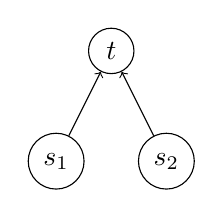
\begin{tikzpicture}[scale=0.7]
%\tikzstyle[thick]
\node at (1,2) [circle,draw](1) {$t$};
\node at (0,0) [circle,draw](2) {$s_1$};
\node at (2,0) [circle,draw](3) {$s_2$};
\path [->] (2) edge node{} (1);
\path [->] (3) edge node{} (1);
\end{tikzpicture}
\caption{基础机关结构}
\label{fig:gadget_basic}
\end{figure}
我们构建的机关如图\ref{fig:gadget_basic}所示,这个机关以节点$s_1,s_2$作为输入,以节点$t$作为输出。
节点$t$有两个入邻居,阈值函数$g(\cdot)$是$\varepsilon$-次模函数。
阈值函数$g(\cdot)$的赋值见等式\ref{eq:func_g}。
\begin{eqnarray*}
\label{eq:func_g}
g(S) =
\left\lbrace
\begin{aligned}
&0,		~ & |S|=0; \\
&\frac{1-\varepsilon}{2},	~ & |S|=1; \\
&1,		~ & |S|=2. \\
\end{aligned}
\right.
\end{eqnarray*}
函数$g(S)$的取值只依赖于输入集合的大小$|S|$,$g(\cdot)$被夹在两个线性的次模函数之间。
$g(\cdot)$自身是一个线性函数在$|S|=1$处向下偏移了$\varepsilon$。
这个基础机关距离与门的性质还很远,接下来我们介绍如何构造更复杂的机关。


我们希望构建出一个机关满足如下性质:
\begin{eqnarray*}
P_a(t) =
\left\lbrace
\begin{aligned}
&1,		~ & \mbox{$s_1,s_2$均被激活}; \\
&o(1),	~ & \mbox{$s_1,s_2$中只有一个被激活}; \\
&0,		~ & \mbox{$s_1,s_2$都未被激活}. \\
\end{aligned}
\right.
\end{eqnarray*}
其中$P_a(t)$是机关的输出节点$t$被激活的概率。
满足这样的性质,当输入节点$s_1,s_2$没有被全部激活时,输出节点$t$很大概率不会被激活。
前面的基础机关在$|S|=1$时,$t$被被激活的概率是$\frac{1-\varepsilon}{2}$,
我们做的就是通过二叉树级联机关放大$\frac{1-\varepsilon}{2}$和$\frac{1}{2}$的差距,
最终使得$|S|=1$时$t$很大概率不被激活,机关的构造如图\ref{fig:gadget_tree}所示。


\begin{figure}[htbp]
\centering
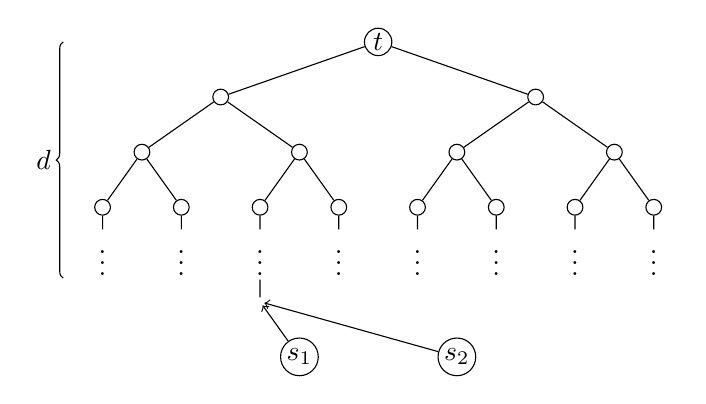
\begin{tikzpicture}[every node/.style={draw,circle,inner sep=1pt}]
% \draw[step=1cm, color=gray] (-5,-5) grid (5,5);
\tikzstyle{level 1}=[sibling distance=40mm,level distance=7mm]
\tikzstyle{level 2}=[sibling distance=20mm]
\tikzstyle{level 3}=[sibling distance=10mm]
\tikzstyle{level 4}=[level distance=6mm]
%\tikzstyle{level 5}=[sibling distance=15mm,level distance=10mm]
\draw[decorate, decoration={brace, mirror}] (-4cm, 0) -- (-4cm,-3cm);
\draw (-4.25cm, -1.5cm) node[draw=none] {$d$};

\node at (-1,-4) [circle,draw](2) {$s_1$};
\node at (1,-4) [circle,draw](3) {$s_2$};
\node {$t$}
	child{
		node{$~$}
		child{
			node{$~$}
			child{
				node{$~$}
				child{node[draw=none] {$\vdots$}
				}
			}
			child{
				node{$~$}
				child{node[draw=none]{$\vdots$}}
			}
		}
		child{
			node{$~$}
			child{
				node{$~$}
				child{node[draw=none]{$\vdots$}
					child{node[draw=none] (leaf_1) {$ $}}
				}
			}
			child{
				node{$~$}
				child{node[draw=none]{$\vdots$}
				}
			}
		}
	}
	child{
		node{$~$}
		child{
			node{$~$}
			child{
				node{$~$}
				child{node[draw=none]{$\vdots$}
				}
			}
			child{
				node{$~$}
				child{node[draw=none]{$\vdots$}}
			}
		}
		child{
			node{$~$}
			child{
				node{$~$}
				child{node[draw=none]{$\vdots$} }
			}
			child{
				node{$~$}
				child{node[draw=none] {$\vdots$}
					%child{node[draw=none] (leaf_2) {$ $}}
				}
			}
		}
	};

\path [->] (2) edge (leaf_1);
\path [->] (3) edge (leaf_1);
\end{tikzpicture}
\caption{二叉树机关$T_\varepsilon$}
\label{fig:gadget_tree}
\end{figure}

在这棵满二叉树中,输出节点$t$是二叉树的根节点,每个节点有一条有向边指向它的父节点。
对每个叶子结点$v$,输入节点$s_1,s_2$会发出有向边指向$v$。
二叉树中每个节点的阈值函数都是前文等式\ref{eq:func_g}定义的$\varepsilon$-次模函数$g(\cdot)$。
整个树状结构被定义为$T_\varepsilon$,$\varepsilon$就是函数$g(\cdot)$距离次模函数的偏移量。
二叉树的深度会在后文定义,我们用$v_i$表示深度为$i$的节点($t$的深度是$1$)。


很显然$s_1,s_2$都被激活时$P_a(t)=1$,$s_1$ or $s_2$都没有被激活时$P_a(t)=0$。
下面我们证明对于深度$d$的二叉树,$s_1,s_2$中只有一个被激活时,输出节点$t$被激活的概率是$O(2^{-d})$。
\begin{lemma}
\label{lem:tree_prob}
对于深度为$d$的机关$T_\varepsilon$,当输入节点只有一个被激活时,
输出节点$t$被激活的概率小于$(\frac{2-\varepsilon}{2})^{d}$。
\end{lemma}
\begin{proof}
对于所有的叶子结点$v_d$,可以得到$P_a(v_d) = \frac{1-\varepsilon}{2}$。
机关$T_\varepsilon$中同一层的节点之前激活与否是互相独立的。
给定一个基础机关(如图\ref{fig:gadget_basic}),如果每个输出节点被激活的概率都是$p$而且互相独立,则输出节点$t$被激活的概率是
\begin{equation*}
\begin{array}{ll}
& P_a(t) \\
= & p^2\times g(2) + 2p(1-p)\times g(1) + (1-p)^2\times g(0) \\
= & p^2 + 2p(1-p)\frac{1-\varepsilon}{2} = p(1-\varepsilon(1-p)).
\end{array}
\end{equation*}
根据这个公式,我们可以写出二叉树上不同深度节点被激活概率的递推公式。
\begin{equation}
\label{eq:recurrence}
P_a(v_i) = P_a(v_{i+1})(1-\varepsilon(1-P_a(v_{i+1}))) <  P_a(v_{i+1})(1-\varepsilon/2)
\end{equation}
不等号的成立是因为树的叶节点满足$P_a(v_d) = \frac{1-\varepsilon}{2}$,而且随着节点所处深度降低,被激活的概率递减。
所以对于树中的任意节点$v$都有$P_a(v) < \frac{1}{2}$。
根据递推公式\ref{eq:recurrence},输出节点$t$被激活的概率为
\begin{equation*}
\label{eq:p_a_t}
 P_a(t) 
=  P_a(v_1) 
<  \frac{1-\varepsilon}{2}(\frac{2-\varepsilon}{2})^{d-1} 
<  (\frac{2-\varepsilon}{2})^{d}.
\end{equation*}
节点$t$被激活的概率$P_a(t) = O(2^{-d})$,随着$d$的增加趋于$0$。
\end{proof}
由引理\ref{lem:tree_prob}我们知道$T_\varepsilon$在输入集合大小为$1$时输出节点被激活的概率是$o(1)$,
$T_\varepsilon$的确是一个两个输入节点的概率与门。


我们已经构造了两个输入节点的树状机关,我们拓展机关$T_\varepsilon$来得到$n$个输入节点的与门$T_\varepsilon^n$。
给定$n$个输入节点$s_1, s_2, \dots, s_n$,我们用节点$s_0$和$s_1$作为输入节点搭建$T_\varepsilon^n$,并令输出节点为$s_{12}$。
接下来可以把节点$s_{12}$和$s_{3}$作为输入节点搭建$T_\varepsilon^n$得到输出节点$s_{123}$。
以此类推,我们得到最终的输出节点$s_{12\dots n}$。
在这个结构中,$s_1, s_2, \dots, s_n$中有节点未被激活时,$s_{12\dots n}$很大概率不会被激活。
如果所有的$T_\varepsilon$都表现出与门的性质,那么整体上就构成了一个$n$个输入节点的概率与门。
由引理\ref{lem:tree_prob}可得深度为$d$的$T_\varepsilon$最多以$(\frac{2-\varepsilon}{2})^{d}$的概率打破与门的规则。
通过Union Bound,$T_\varepsilon^n$在输入中有未激活节点时输出节点被激活的概率至多为$n(\frac{2-\varepsilon}{2})^{d}$。
$T_\varepsilon^n$一共包含$n\times(2^d-1) = n2^d-n$个节点。





先说m们,然后下一节说sketch
We then construct a multi-input probabilistic-AND gate based on our probabilistic-AND gate by the similar method to construct multi-input-AND gate based on 2-input-AND gate. Finally, we show if influence maximization problem can be approximated beyond the ratio shown above, we can solve the set cover problem in polynomial time. The main idea is as follows. For any set cover instance, we will put all elements to be the input of our multi-input-probabilistic-AND gate, and connect the output with a large number of additional nodes. Thus, if $k$ sets can cover all elements, all of those addition nodes will be activated, on contrast, if one of the elements cannot be covered, almost all of the additional nodes will remain inactivated.

\subsection{基于Set Cover的不可近似性规约}
在本节基于概率与门,我们证明定理\ref{the:inapp}。
前面一节基于二叉树级联得到的2-输入概率与门$T_\varepsilon$,我们构造了$n$个输入的概率与门$T_\varepsilon^n$。
在接下来的证明中,我们说明如果$\varepsilon$-次模逼近网络中影响力最大化算法可以取得超过给定的近似比,那么Set Cover问题就可以在多项式时间内被解决。
证明的整体思路是对于集合覆盖的一个实例,我们构造一个网络。网络中代表元素的点是$T_\varepsilon^n$的输入,
然后把$T_\varepsilon^n$的输出点连接到数量很大的额外节点。
因此,当$k$个集合可以覆盖住所有元素时,额外节点都会被激活。否则,$T_\varepsilon^n$的输出大概率不会被激活,额外节点都未被激活。
\begin{proof}[定理\ref{the:inapp}]
我们考虑一个基于集合覆盖构建出的图,在这个网络中影响力最大化算法的近似比不能超过给定的值,否则集合覆盖问题就将被解决,这就导致矛盾。
令$e_1, e_2, \dots, e_n$为表示集合覆盖实例中$n$个元素的节点,$s_1, s_2, \dots, s_m$为表示$m$个集合的节点。
我们可以假定$m<n$,因为当$m\geq n$时,我们可以添加$m$个冗余节点(dummy nodes),他们分别被$m$个集合覆盖。
原始的集合覆盖有$k$个集合的解时,新的集合覆盖问题就有$m+k$个集合的解。
集合节点$s_i$会持有指向所有它覆盖元素节点的有向边,而且所有元素节点$e_j$的阈值函数是$f_{e_j}(1)=1$。
也就是说只要覆盖$e_j$的集合节点中至少有一个被激活,$e_j$就会被激活。
接下来们增加$n^\alpha$个与门节点$x_1, x_2, \dots, x_{n^\alpha}$,$\alpha$的值在后文确定。
在节点$x_k$和元素节点$e_1, e_2, \dots, e_n$之间插入$n$输入概率与门$T_\varepsilon^n$,$x_k$是输出节点,如图\ref{}所示。

然后对于参数$\alpha$,我们对每一个与门节点$x_k$添加$n^\alpha$个冗余节点$c_1, c_2, \dots, c_{n^\beta}$。
对每个冗余节点$c_l$,阈值函数同样是$f_{c_l}(1)=1$。
构建好的图中有集合节点$s_i$,元素节点$e_j$,与门节点$x_k$,冗余节点$c_l$以及构成概率与门的节点。
除了构成概率与门的节点阈值函数是等式\ref{eq:func_g}定义的$\varepsilon$-次模毕竟函数,其余节点的阈值函数都是次模函数。





Here we calculate the depth of $T_\varepsilon$ in order to make sure that the $n^\alpha$ $T_\varepsilon^n$ are all AND gate with high probability.
Again we apply Union Bound to calculate the probability upper bound of at least one $T_\varepsilon^n$ fails
--- $n^{1+\alpha}(\frac{2-\varepsilon}{2})^{d}$.
We set $d = (1+\alpha+\lambda)\log n / \log{\frac{2}{2-\varepsilon}}$,
so all the $T_\varepsilon^n$ observe the rule of AND gate with probability at least $1-n^{-\lambda}$.

If we can find $k$ sets that cover all the $n$ elements, then we just select the $k$ nodes corresponding to the $k$ sets as seed nodes.
Then the seed nodes will activate nodes $e_1, e_2, \dots, e_n$ and then all nodes in gadgets $T_\varepsilon^n$ will become activated.
Finally, all the child nodes of $x_1, x_2, \dots, x_{n^\alpha}$ become activated, and totally $k+n+n^{\alpha+1}(2^d-1)+n^{\alpha\beta} \geq n^{\alpha\beta}$ nodes become activated in total, while the graph consists of $N = m+n+n^{\alpha+1}(2^d-1)+n^{\alpha\beta}$ nodes, nearly all nodes are activated.
On the other hand, if there is no solution of size $k$ for this set cover problem, we can not activate all element nodes $e_i$.
During the influence spread of a given target nodes,
none of $x_1, x_2, \dots, x_{n^\alpha}$ will become activated with probability al least $1-n^{-\lambda}$.
Under this circumstance, we can select nodes labeled with $x$ as seeds or just try to activate more nodes $e_i$.
Totally we can just activate at most $k+n+kn^{\beta}$ nodes if we choose $x_i$ as seeds.
Otherwise we can assume that at most $n-1$ elements are covered and all gadget nodes are activated.
In this case $k+n-1+n^{\alpha+1}(2^d-1)$ nodes will become active if all probabilistic AND gate work perfectly.
One the other hand if these $T_\varepsilon^n$ fails with probability at most $n^{-\lambda}$, we just assume that all the nodes will become activated eventually.
We can set $n^{\beta} = n^{\alpha-1} \cdot 2^d \cdot n^{\delta}$ for $\delta>0$ to 
ensure that the fraction of gadget nodes and dummy nodes is slightly less than $n^{\frac{1}{\alpha-1}}$. 
When $n$ is large enough the influence size we obtain  
is less then $kn^{\beta} \leq n^{\beta+1}$ or $n^{\alpha+1}2^d$ w.h.p. when Set Cover is not solved.
For any influence maximization algorithm,
there exists a graph of $N$ nodes where at most $n^{\alpha+1}(2^d-1)$ nodes have $\varepsilon$-almost submodular threshold function,
for any result obtained,
with probability at least $1-n^{-\lambda}$,
the influence size is less than $1/n^{\alpha-1}$ of $\sigma(S^*)$,
unless we can solve Set Cover problems within polynomial time.
Here $N \geq n^{\alpha+\beta}$, $d = (1+\alpha+\lambda)\log n / \log{\frac{2}{2-\varepsilon}}$, $\beta = (\alpha+1) + (1+\alpha+\lambda) / \log{\frac{2}{2-\varepsilon}} + \delta$.
We can substitute the parameter into the conclusion, we obtain that $\forall \alpha>1, \lambda>0, \delta>0$, there exists
$b = 1/\log{\frac{2}{2-\varepsilon}}$,
$\varphi= \frac{ \min\{\alpha-1, \lambda\}}{2\alpha+\delta-1+b(1+\alpha+\lambda)}$ and
$\gamma =\frac{\alpha+1+b(1+\alpha+\lambda)}{2\alpha+\delta-1+b(1+\alpha+\lambda)}$,
for any influence maximization algorithm based on measg{gamma},
there exists an instance of graph,
the approximation ratio is less than $n^{-\gamma}$.
Notice that $\varphi \geq \frac{\gamma}{3+3b}$ when we set $\alpha=\lambda+1$ and $\lambda \geq 1$.
$\gamma$ ranges in $(0,1)$, hence the theorem follows.
\end{proof}

\section{近似算法}


\section{本章小结}









%\chapter{总结与展望}
\section{研究工作总结}
信息化社会的到来,社交网络的用户量在爆发式增长。
社交网络中信息的扩散机制和基于社交网络的营销策略越发成为研究热点。
在本文中,我们研究学习了社交网络中一些非次模的问题,主要是基于非次模的阈值函数。
之前的研究大多集中在次模阈值函数和次模影响力函数,我们的研究和他们大不相同。
根据前人的实验观察,我们研究了两类非次模函数----$\varepsilon$-次模逼近函数和$k$-激活函数,
然后分别讨论了基于$\varepsilon$-次模逼近函数的影响力最大化问题和基于$k$-激活函数的小世界网络路由问题。
首先我们证明了尽管$\varepsilon$-次模逼近函数和次模函数很接近,
在有$\varepsilon$-次模逼近节点的图中影响力最大化问题依然很难近似。
通过构造概率与门并从NP完全问题集合覆盖规约,我们证明了
$n$个节点的图中只要有$n$的多项式个$\varepsilon$-次模逼近节点影响力最大化算法就无法做到$log$近似。
然后我们通过把$\varepsilon$-次模逼近函数替换成次模的上界或者下界,转化问一个次模优化问题,
设计了近似算法\textsf{Galg-U}和\textsf{Galg-L}。
基于概率空间映射,我们证明了这个近似算法的近似比为$(1-\frac{1}{e})(1-\varepsilon)^c$,
其中$c$是$\varepsilon$-次模逼近节点的个数。
接下来我们研究了Kleinberg小世界网络中,基于$k$-激活函数的路由。
本文定量地研究了从两个相邻的种子节点开始去感染一个网格上最远目标$t$需要的步数,也就是路由时间。
在每一步,只有一个节点会被激活,选择被激活节点的策略是分散式的,也就是路由选择策略只能基于当前被激活的节点发出的强连接和弱连接。
复杂路由比较像社交网站上最近提出的一个应用:主动交友,主动交友是指在像Facebook、人人网等社交网站上通过添加一些中间好友来增加目标接受自己好友请求的概率\cite{YangHLC13}。
本文指出与$k$-激活传播不同,对于所有的$\alpha$,$k$-激活路由时间均有$n$的多项式的下界,即使每一步允许激活多个节点。


本文的最后实现了算法\textsf{Galg-U}和\textsf{Galg-L}和其他基准算法,
并且在真实的社交网络{\em NetHEPT}、{\em Flixster}和{\em DBLP}上测试对比了算法和其他基准算法效果。
在小数据集上,\textsf{Galg-U}和\textsf{Galg-L}算法效果比\textsf{Greedy}稍好,
但是算法的运行时间要少很多,因为\textsf{Galg-U}和\textsf{Galg-L}可以利用一些次模上下界利用\textsf{TIM}算法加速。
在较大的网络{\em Flixster}和{\em DBLP}上,\textsf{Galg-U}和\textsf{Galg-L}均比其他基准算法要好。
而且在$\varepsilon$-次模逼近节点个数达到总结点个数$\frac{1}{3}$时,算法的表现依然很好。
这说明\textsf{Galg-U}和\textsf{Galg-L}不仅仅有理论近似比保证,实际中运行效果也很好。




\section{未来工作的展望}
在影响力最大化问题上,本文目前的研究主要集中在$\varepsilon$-次模逼近函数,
但是对于那些和次模函数相距很远的非次模阈值函数,我们还不知道如何设计有效的算法。
此外,我们提出的算法在实验中采用了逆向可达集合进行加速。
并不是所有的次模函数都可以使用逆向可达集合,
研究哪些函数可以使用逆向可达集合进行加速或者设计基于次模函数的加速算法也是新的研究方向。

其次,在研究$k$-激活路由时,为了更好地应用延迟选择原则,本文采用了有向Kleinberg小世界网络模型。
因为每个节点的弱连接平均数量仍为常数,有向小世界网络和无向小世界网络中$k$-激活路由的效率应该不会相差太多。
后续的工作希望可以研究$k$-激活路由在无向Kleinberg小世界网络中的性能。
未来也可以研究在什么样结构的网络中$k$-激活路由可以很快找到目标,探讨$k$-激活路由在其他小世界模型中的执行效率。
为$k$-激活路由寻找更广泛的应用场景也是未来需要进行的工作之一。



%\ICTbackmatter{\bibliography{bib/ref}\nocite{*}}
\ICTbackmatter{\bibliography{bib/ref}}
%\bibliography{bib/ref}
%
\begin{thanks}


在完成硕士学位论文之际,我在此向所有支持我、关心我的老师、师兄、同学和家人致以最衷心的感谢。
是你们的帮助,让我能够顺利完成毕业设计。
感谢中科院计算所前瞻实验室所对我的支持,感谢算法与复杂性课题组,
让我能够在一个科研环境优越的地方研究学习。


首先十分感谢我的指导教师孙晓明研究员。
自从我研一进入实验室以来,孙老师在科研、学习、生活方面给了我非常多的帮助。
感谢孙老师对我论文的选题、设计、完成以及论文修改等各个方面给予的悉心指导。
我也要感谢答辩组的各位老师,卜东波老师、和张家琳老师,你们在开题答辩和中期检查时都给提出了我非常重要的指导意见,
让我对自己的工作有了更深刻的认识,得到了新的启示。

我还要感谢在微软亚洲研究院实习时对我科研进行过指导的陈卫老师,
每周和你的讨论我都收益颇多,你对我在科研部分给予了细致的指导,在这里衷心地感谢你对我的教导。


感谢我的好朋友曾钢同学,毕设过程中我们互相鼓励,谢谢你的一路支持。
也感谢我的舍友顾茂杰和朱良昌以及实验室的岑武斌同学,是你们陪伴我走过了毕设的日子,谢谢你们对我的鼓励和支持。
我还要感谢实验室的师兄师姐们,感谢你们对我毕业设计提出了宝贵的意见,耐心的解答我们的疑惑。

在此,也要感谢我的家人对我的支持和鼓励,特别是父亲和母亲,你们的鼓励永远让我充满动力。

最后要感谢我的女朋友,在研究生阶段,让我踏实安心的工作,默默地支持我,谢谢你一直以来的陪伴!


感谢所有给予过我帮助与支持的老师同学们!


\end{thanks}

%
\begin{resume}

\begin{resumelist*}{教育经历}
\resumelistitem 20010年9月---~2014年7月,北京航空航天大学,计算机学院,学士
\resumelistitem 2014年9月---~2017年7月,中国科学院,计算技术研究所,硕士
\end{resumelist*}

\begin{resumelist}{【攻读硕士学位期间发表的论文】}
\resumelistitem Wei Chen, Qiang Li, Xiaoming Sun, Jialin Zhang. The Routing of Complex Contagion in Kleinberg's Small-World Networks. Annual International Computing and Combinatorics Conference, 2015: 307-318.
\end{resumelist}

\begin{resumelist}{【攻读硕士学位期间参加的科研项目】}

\resumelistitem 国家重点基金

\end{resumelist}

\end{resume}

\end{document}
